\documentclass[11pt, a4paper]{article}
\usepackage{fullpage}
\usepackage{pythontex}
\usepackage{subfiles}
\usepackage[parfill]{parskip}
\usepackage{listings}
\usepackage{color}
\usepackage{graphicx}
\usepackage{subcaption}
\usepackage{verbatim}
\usepackage{cite}
\usepackage{caption}
\usepackage{subcaption}
\usepackage[hidelinks]{hyperref}
\hypersetup{
    pdftitle={Analysis - Simulating disease spread through Cellular Automata and the SIR model DRAFT},
    pdfauthor={Zebedee Marsh},
    bookmarksnumbered=true,     
    bookmarksopen=true,         
    bookmarksopenlevel=1,        
    pdfstartview=Fit,           
    pdfpagelayout=TwoPageRight,
    pdftex
}

\graphicspath{ {images/} }

\definecolor{dkgreen}{rgb}{0,0.6,0}
\definecolor{gray}{rgb}{0.5,0.5,0.5}
\definecolor{mauve}{rgb}{0.58,0,0.82}

\lstset{frame=tb,
  language=Python,
  aboveskip=3mm,
  belowskip=3mm,
  showstringspaces=false,
  columns=flexible,
  basicstyle={\small\ttfamily},
  numbers=none,
  numberstyle=\tiny\color{gray},
  keywordstyle=\color{blue},
  commentstyle=\color{dkgreen},
  stringstyle=\color{mauve},
  breaklines=true,
  breakatwhitespace=true,
  tabsize=3
}

% \bibliography{references.bib}
\author{Zebedee Marsh}
\title{Analysis - Simulating disease spread through Cellular Automata and the SIR model DRAFT}

\begin{document}
    
\maketitle
\tableofcontents
\newpage

\section{Introduction}
Since 1999, there have been 11 major disease outbreaks across the globe, eight of which involved thousands of cases. To effectively control an outbreak and ultimately stop it in its tracks, it's current and past states must be analysed so it's spread can be predicted, which is essential in influencing how governments should deal with such a threat.

This is currently being seen in how the UK government is dealing with COVID-19, where a balance between a total lockdown and total freedom needs to be struck to control how the virus spreads. This balance is essential in allowing businesses to continue operating, keeping the economy afloat and allowing people their freedoms to do what they want.

My project aims to provide a starting point for where a disease outbreak can be modelled either by cellular automata or the SIR model, which can be used in an educational environment to teach people about the spread of diseases. A user will be able to input custom parameters according to the disease they are trying to simulate and be able to introduce special events such as a partial or permanent lockdown, to be able to see how the disease spread could change. A user should also be able to compare the two different ways of simulating a disease.

Source: https://sundial.csun.edu/156361/news/a-timeline-of-outbreaks-from-2000-to-present/

\section{Initial objectives}
These objects represent my initial aims of what this project should be able to do. These may change later on throughout this project.
\begin{itemize}
    \item Simulate the spread of a disease using the SIR model
    \item Simulate the spread of a disease using the Cellular Automata model
    \item Input custom parameters or use default values (from a previous disease) including infection rate, incubation period and death rate for the SIR model
    \item Input custom parameters or use default values (from a previous disease) relating to the number and infectivity of cells for the CA model
    \item Set a quarantine period or introduce a vaccine (therefore limiting disease transmission)
    \item Click on a graph and show statistics from that point in time
    \item Export graphs produced as png
    \item Upload past simulation results into the program to generate a graph from that previous simulation
    \item Be able to compare graphs of two different diseases

\end{itemize}

\section{Potential user}
Mr Bliss - Biology teacher at Abingdon School
As this model provides a starting point for modelling disease outbreak, it’s most effective use would be in an education environment, where it is used to teach people about how disease can spread and how changes in parameters such as the infection rate, recovery rate, time of infection and immunity can affect how effectively a disease is transmitted throughout a cohort. 



\section{How the problem was researched}
To first understand how I could make this project, I had to research the two main methods of modelling disease spread, the SIR model and Cellular Automata. Once I got the basic idea of how each model worked, I further researched how I could implement these in Python, as well as looking at how to use some Python libraries to help me.
\begin{itemize}
    \item Find out how SIR and Cellular Automata work
    \item Research how to implement SIR and Cellular Automata in code
    \item Learn how to use the Matplotlib library to draw graphs for my disease models
    \item Learn how to use Pandas to export data to an external file
    \item Learn how to use Tkinter to create a GUI interface and multiple pages
    \item Learn how to create, use and modify an SQL database using Sqlite3
\end{itemize}
\subsection{The SIR model}
The SIR model is a simple disease spread model which uses differential equations to determine the number of people in three categories, the susceptible, the infected and the recovered. The susceptible population represent those who can become infected a disease, the infected population represent those currently infected with the disease who are able to spread it to other people and the recovered population represent those who are no longer infected. In some models, people in the recovered population can be infected again.
\subsubsection{Equations for the SIR model}

\textbf{People in each group}

\(S = S(t) \) - number of susceptible individuals

\(I = I(t) \) - number of infected individuals

\(R = R(t) \) - number of recovered individuals


\textbf{The Susceptible equation}
\[ \frac{dS}{dt}=\frac{-\beta S(t)I(t)}{N} \]
where \(\beta\) is the rate at which infections occur (a positive constant)


\textbf{The Infected equation}
\[ \frac{dI}{dt}=\frac{\beta S(t)I(t)}{N}-\gamma I(t) \]
where \(\gamma\) is the rate at which people recover


\textbf{The Recovered equation}
\[ \frac{dR}{dt}=\gamma I(t) \]


\textbf{Model without vital dynamics}
\[ \frac{dS}{dt} + \frac{dI}{dt} + \frac{dR}{dt} = 0 \]
As this model doesn't take into account vital dynamics ie. people aren't added through birth or removed through death, the sum of all the changes is constant and equal to 0


\subsection{The Cellular Automata model}
The basic idea of cellular automata that there there is a collection of cells with a finite set of states. Every new generation, the state of a cell can be changed depending on the state of it's neighbouring cells. 

\subsubsection{My implementation of CA}
\begin{itemize}
    \item Cells move randomly within a grid. Most cells will be susceptible but some will be infected
    \item If a susceptible cell comes in close range to an infected cell, there is a chance that that susceptible cell will be come infected
    \item Infected cells are only infected for a certain period of time, so after a certain number of generations the cell will no longer be infected and will be in the recovered category
\end{itemize}
\newpage
\section{Prototyping of code}

\subsection{The scientific models}
\subsubsection{Elementary cellular automata}
My initial cellular automata model was very basic and only worked on a 1D line. The shape of each new line would be decided by looking at the previous line and applying a ruleset to it.
\begin{lstlisting}
class CA:
    def __init__(self, width, generations):
        self.ruleset = [0, 1, 1, 1, 1, 0, 1, 1]
        self.width = width
        self.cells = [0] * width
        self.new_cells = [None] * width
        self.cells[int((width / 2) - 1)] = 1
        self.generations = generations
        self.cell_timeline = []

    def rules(self, a, b, c, i):
        index = int((a + b + c), 2)
        ruleset = [0, 1, 0, 1, 1, 0, 1, 0]
        self.new_cells[i] = ruleset[index]

    def draw(self):
        output = ""
        for cell_state in self.cell_timeline:
            for element in cell_state:
                if element == 0:
                    output += " " + " "
                else:
                    output += "X" + " "
            print(output)
            time.sleep(0.1)
            output = ""

    def ca(self):
        for gen in range(self.generations):
            for i in range(self.width):
                a = str(self.cells[((i - 1) % self.width)])
                b = str(self.cells[i])
                c = str(self.cells[((i + 1) % self.width)])
                # print(a,b,c)
                self.rules(a, b, c, i)
            self.cells = self.new_cells
            self.cell_timeline.append(self.cells)
            self.new_cells = [None] * self.width
        self.draw()

ca = CA(100, 100)
ca.ca()
\end{lstlisting}
\textbf{The result of elementary cellular automata}

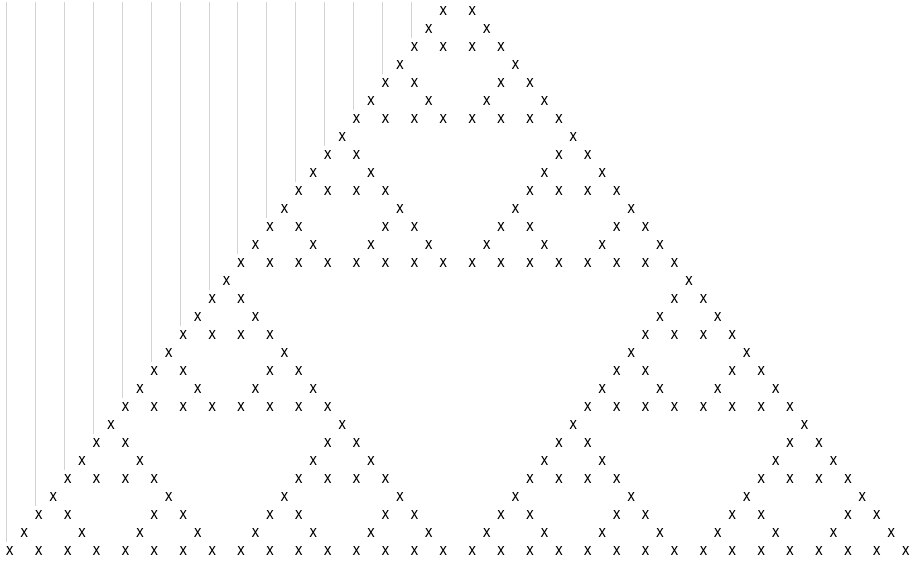
\includegraphics[width=\textwidth]{eca.png}

\subsubsection{Basic SIR model}
My starting block for the SIR model was a function which calculated the rate of change of the susceptible, infected and recovered population. 
\begin{lstlisting}
def eqns(y0, t, beta, gamma):
S, I, R = y0
dsdt = -(beta * S * I) / N  # rate of change of susceptible individuals
didt = ((beta * S * I) / N) - gamma * I  # rate of change of infected individuals
drdt = gamma * I  # rate of change of recovered individuals
return dsdt, didt, drdt
\end{lstlisting}

\subsection{External library testing TBD}
\subsubsection{Tkinter}
My intial prototying for tkinter was done with the help of a YouTube video which focused on having multiple tkinter pages in a single file.
Link: https://youtu.be/jBUpjijYtCk

This prototype allowed there to be multiple Tkinter windows which could be switched between by a button click. The way this method worked was by removeing and adding widgets depending on which page should be shown. Although this method may have worked for me, in the final project I went with destroying a Tkinter window and starting a completely new one when a user wanted to switch, as the code for this was easier to understand and write. 

\begin{lstlisting}
import tkinter as tk


class Gui(tk.Tk):

    def __init__(self, *args,
                    **kwargs):  # *args - pass through any number of variables; **kwargs - pass through dictionaries
        tk.Tk.__init__(self, *args, **kwargs)  # initialising tkinter
        container = tk.Frame(self)  # the frame of the window
        container.pack(side="top", fill="both", expand=True)
        container.grid_rowconfigure(0, weight=1)  # 0 sets minimum size, weight shows priority
        container.grid_columnconfigure(0, weight=1)
        self.frames = {}  # allows application to open different types of pages easily

        for F in (StartPage, PageOne):  # all pages need to be listed here
            frame = F(container, self)
            self.frames[F] = frame  # saving classes to dictionary, "loading it in"
            frame.grid(row=0, column=0, sticky="nsew")

        self.show_frame(StartPage)  # start page is shown first

    def show_frame(self, cont):
        frame = self.frames[cont]  # looks for cont in dict
        frame.tkraise()  # which is then raised


class StartPage(tk.Frame):

    def __init__(self, parent,
                    controller):  # parent class is Gui, controller class is main class, allowing show_frame to be called
        tk.Frame.__init__(self, parent)

        label = tk.Label(self, text="Start Page")
        label.pack(pady=10, padx=10)
        button1 = tk.Button(self, text="Page 1", command=lambda: controller.show_frame(PageOne))
        button1.pack()


class PageOne(tk.Frame):

    def __init__(self, parent, controller):
        tk.Frame.__init__(self, parent)

        label = tk.Label(self, text="This is page 1")
        label.pack(pady=10, padx=10)
        button2 = tk.Button(self, text="Start Page", command=lambda: controller.show_frame(StartPage))
        button2.pack()


app = Gui()
app.mainloop()
\end{lstlisting}
\textbf{The result}

\begin{figure}
    \centering
    \begin{minipage}{.5\textwidth}
      \centering
      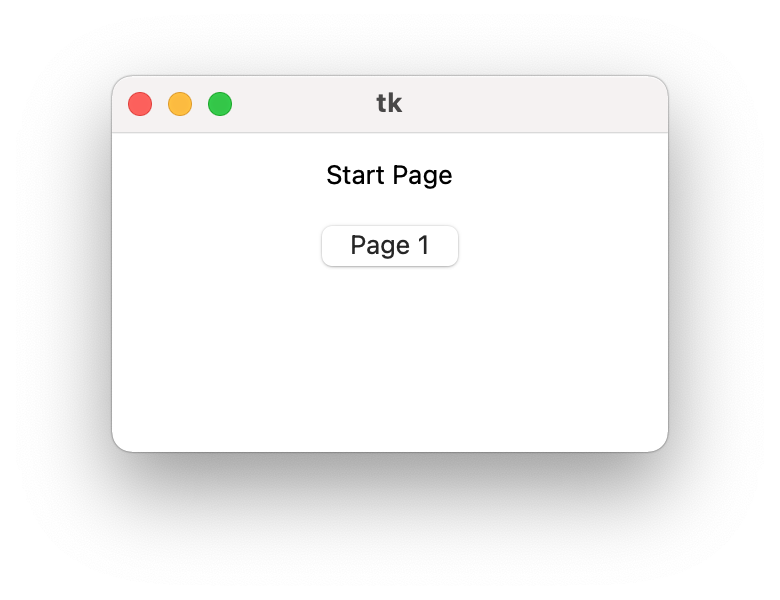
\includegraphics[width=\linewidth]{p_tk_start.png}
      \captionof{figure}{Start Tkinter window}
      \label{fig:test1}
    \end{minipage}%
    \begin{minipage}{.5\textwidth}
      \centering
      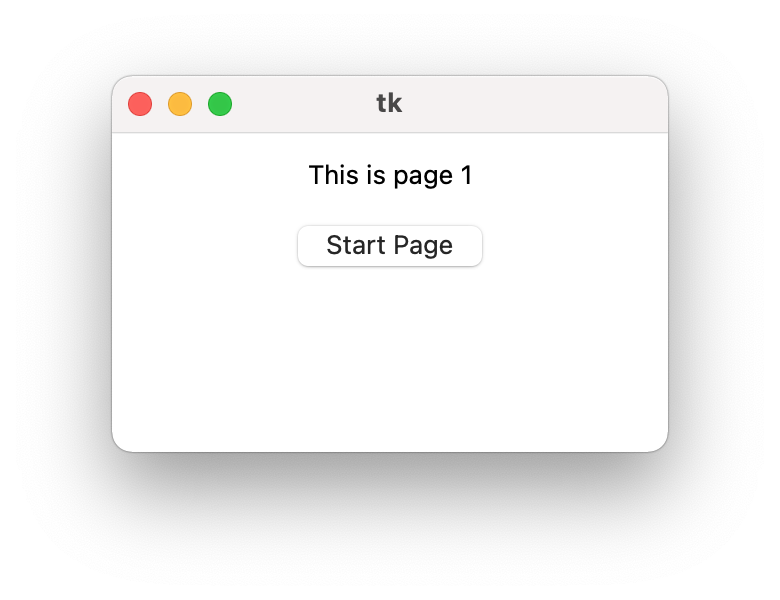
\includegraphics[width=\linewidth]{p_tk_p1.png}
      \captionof{figure}{Page 1 Tkinter window}
      \label{fig:test2}
    \end{minipage}
\end{figure}


\subsubsection{Matplotlib - FuncAnimation}
The initial way I tried to update a graph with new values was by deleting the graph and plotting a new one. Funcanimation provided an easier way to do this, with the option of saving the animation as a video which was one of the objectives for my project. This prototype shows how a line graph works with funcanimate.

It works for both line graphs and scatter graphs
\begin{lstlisting}
    import matplotlib.pyplot as plt
    from matplotlib.animation import FuncAnimation
    from itertools import count
    import random
    
    x_full = [[229, 29, 52, 90, 78], [228, 29, 52, 90, 79], [229, 28, 53, 89, 79], [228, 27, 52, 90, 78], [227, 28, 51, 89, 79], [227, 27, 50, 88, 78], [226, 28, 51, 88, 79], [227, 29, 51, 89, 79], [227, 30, 51, 90, 79], [228, 30, 51, 90, 79], [229, 30, 50, 89, 78], [228, 30, 49, 90, 79], [228, 30, 50, 89, 78], [228, 31, 50, 88, 78], [229, 32, 49, 87, 78], [230, 33, 50, 87, 77], [230, 34, 50, 88, 76], [231, 35, 51, 87, 75], [232, 36, 50, 87, 74], [232, 37, 51, 86, 74]]
    y_full = [[37, 23, 94, 195, 90], [37, 22, 93, 194, 89], [36, 22, 94, 195, 88], [36, 22, 95, 194, 88], [35, 22, 94, 195, 88], [36, 22, 95, 196, 89], [35, 21, 94, 197, 90], [34, 20, 94, 196, 91], [34, 20, 94, 197, 90], [35, 19, 94, 196, 90], [35, 18, 95, 197, 89], [35, 18, 94, 198, 88], [35, 19, 93, 197, 89], [35, 20, 94, 196, 90], [34, 20, 95, 196, 90], [33, 19, 95, 195, 90], [33, 19, 96, 196, 91], [33, 20, 95, 196, 90], [32, 20, 94, 195, 90], [31, 19, 93, 194, 91]]
    
    x_vals = []
    y_vals = []
    
    index = count()
    
    def animate(i):
        x_vals.append(next(index))
        y_vals.append(random.randint(0,5))
        plt.plot(x_vals, y_vals)
    
    ani = FuncAnimation(plt.gcf(), animate, interval=10)  # get current figure, function, interval
    plt.show()
\end{lstlisting}

\textbf{The result}

\begin{figure}
    \centering
    \begin{minipage}{.5\textwidth}
      \centering
      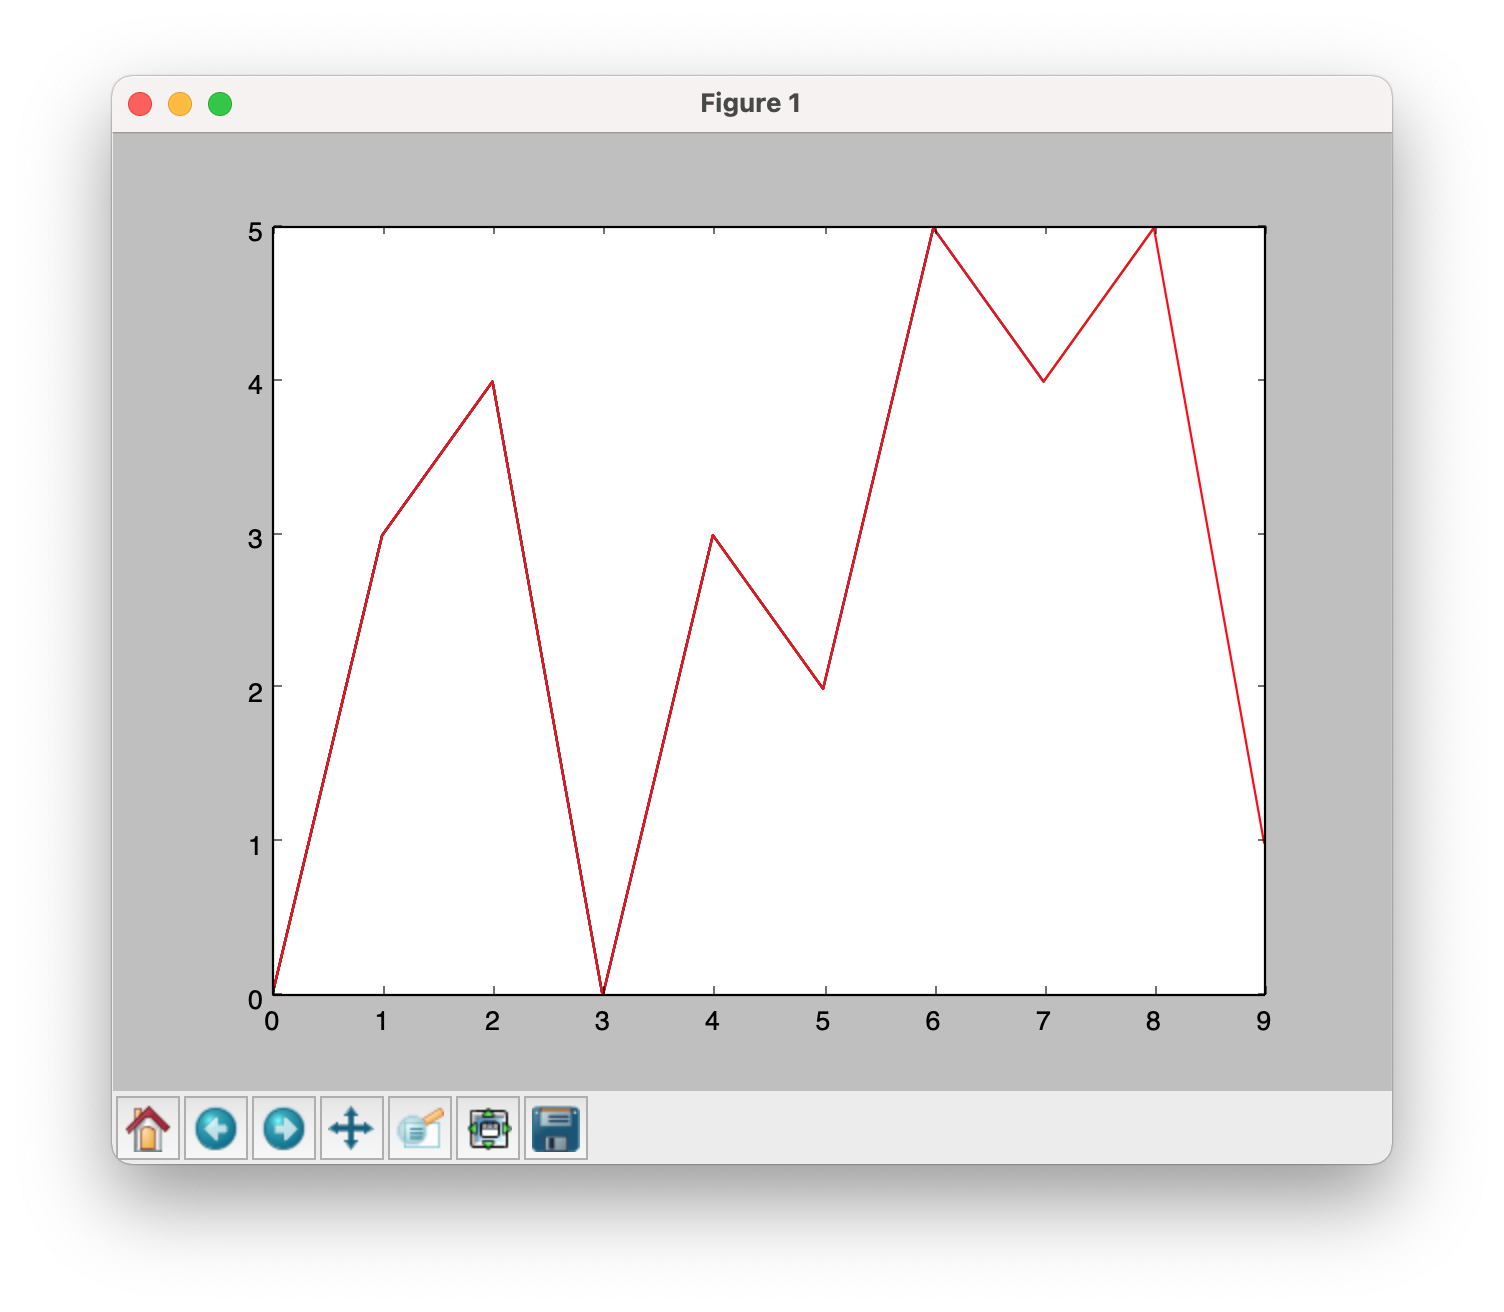
\includegraphics[width=\linewidth]{p_fa_1.png}
      \captionof{figure}{Graph 1}
      \label{fig:test1}
    \end{minipage}%
    \begin{minipage}{.5\textwidth}
      \centering
      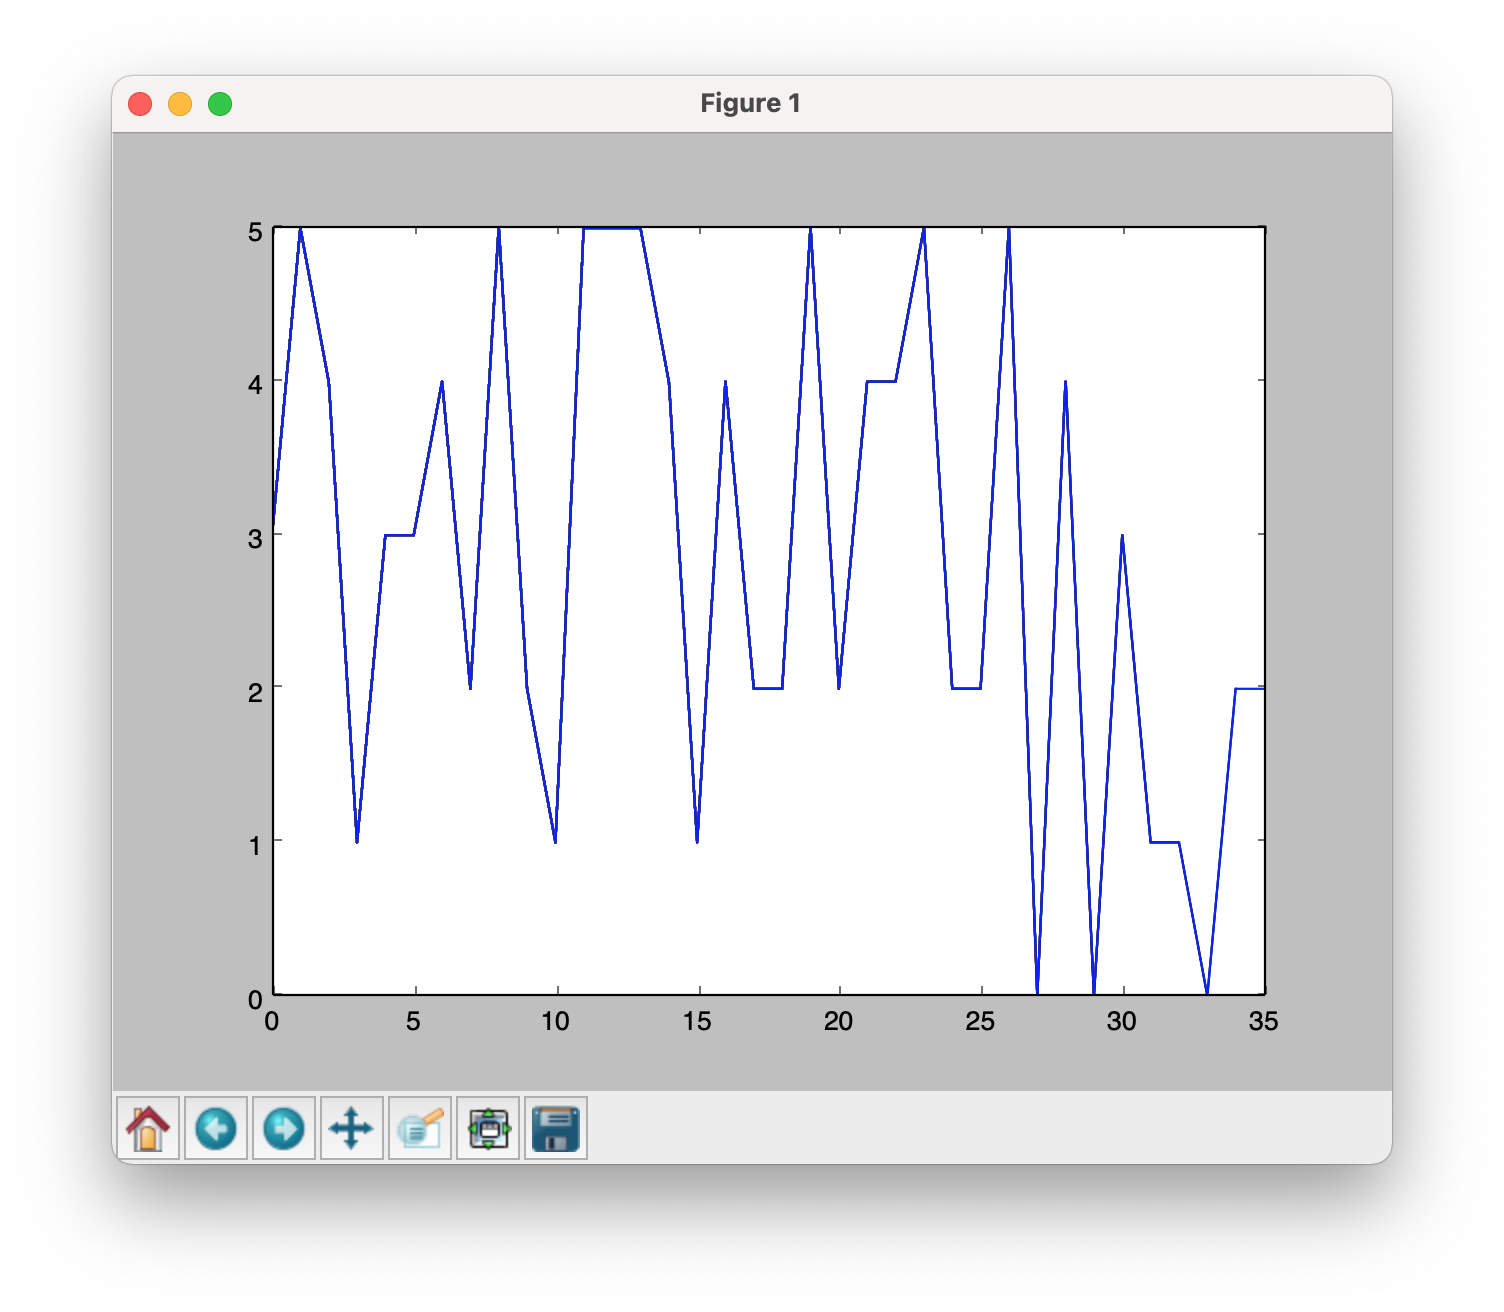
\includegraphics[width=\linewidth]{p_fa_2.png}
      \captionof{figure}{Graph 2}
      \label{fig:test2}
    \end{minipage}
\end{figure}

\begin{figure}
    \centering
    \begin{minipage}{.5\textwidth}
      \centering
      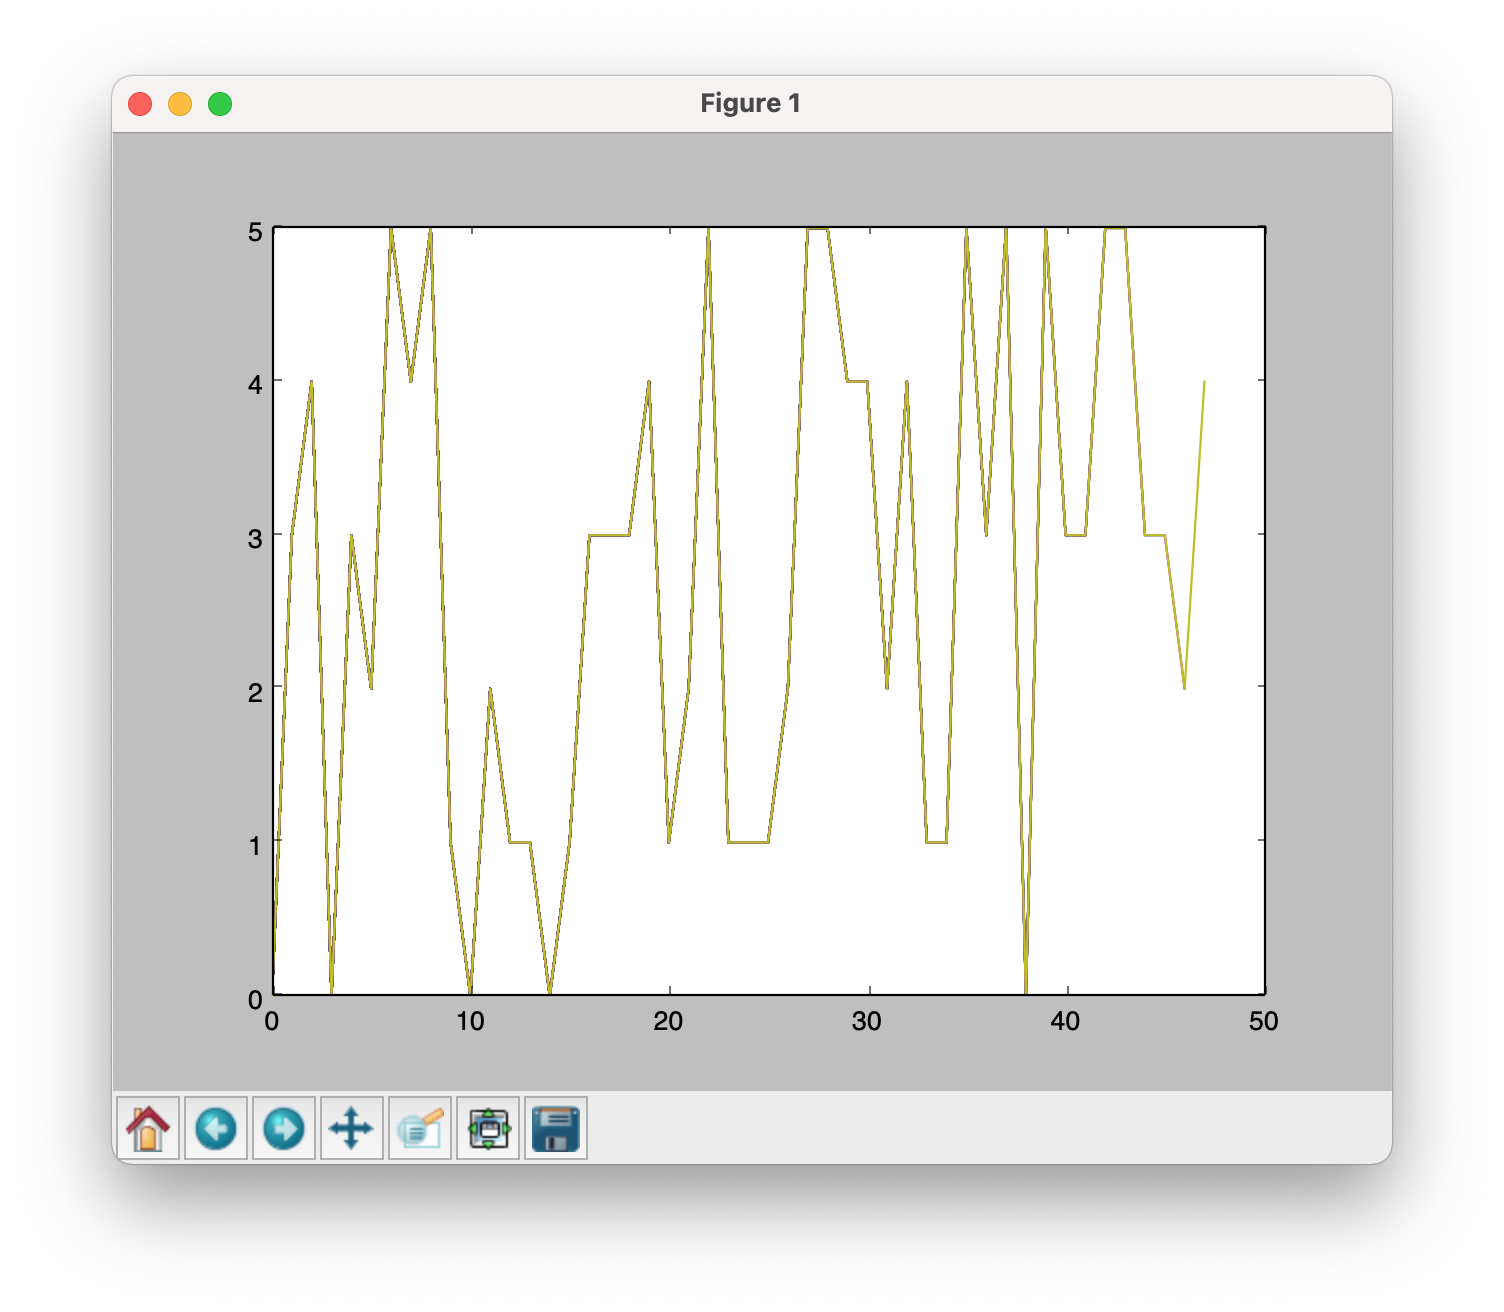
\includegraphics[width=\linewidth]{p_fa_3.png}
      \captionof{figure}{Graph 3}
      \label{fig:test1}
    \end{minipage}%
    \begin{minipage}{.5\textwidth}
      \centering
      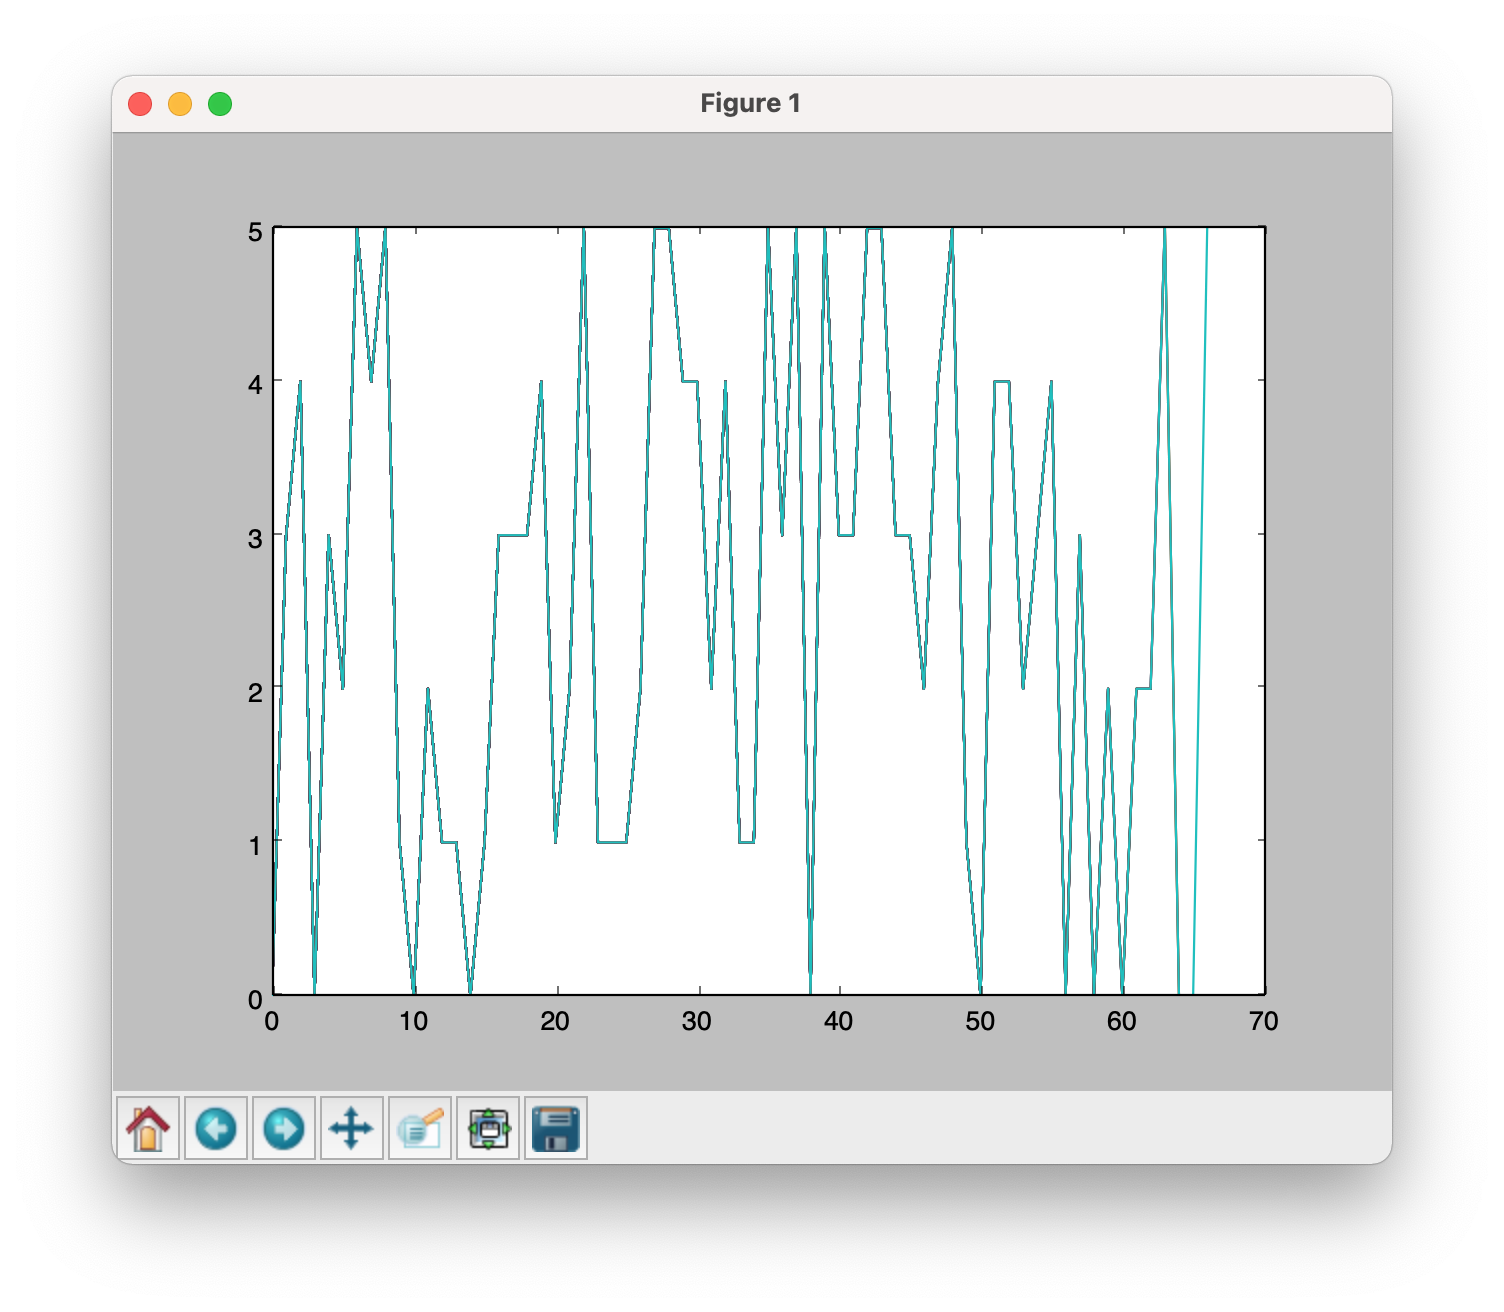
\includegraphics[width=\linewidth]{p_fa_4.png}
      \captionof{figure}{Graph 4}
      \label{fig:test2}
    \end{minipage}
\end{figure}

\subsubsection{Pandas}
I used Pandas to help export the data generated using the SIR model. This allowed me to generate an excel file with appropriate column names, which could possibly be used later for data analysis
\begin{lstlisting}
def export_to_excel():
data = {'Time': timearray,
        'S': solver_result[0],
        'I': solver_result[1],
        'R': solver_result[2]}

df = pd.DataFrame(data, columns=['Time', 'S', 'I', 'R'])
name = "output" + str(f) + ".xlsx"
df.to_excel(name, sheet_name='output')
\end{lstlisting}
\begin{center}
    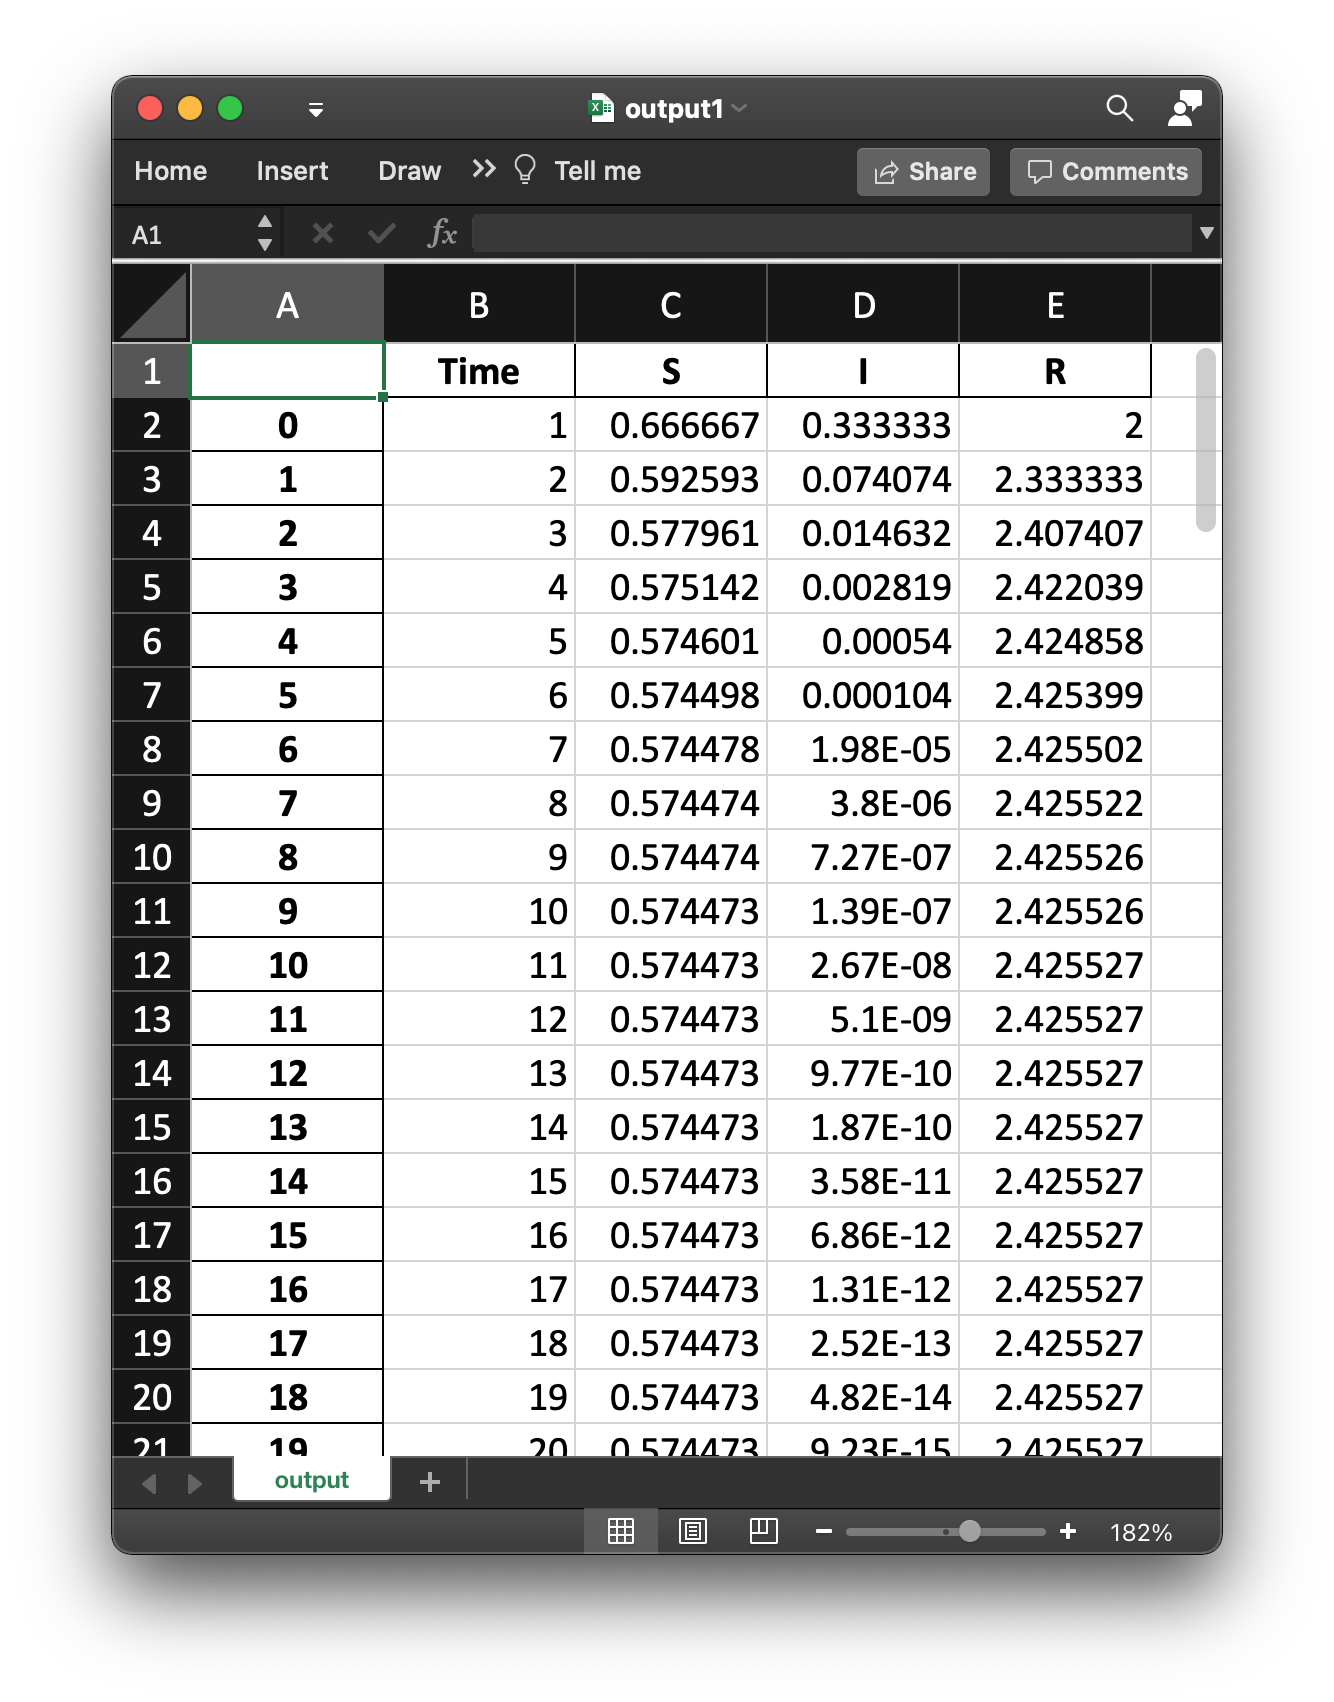
\includegraphics[height=10cm, width=\linewidth, keepaspectratio]{p_pan.png}
\end{center}

\subsubsection{Pygame}
One of the options I considered to simulate and show my Cellular Automata simulation was Pygame. With Pygame I would be able to easily create cells which could move randomly in a set space, and using Pygame's collision method I could detect if cells touched. In the end I decided against this method as although it may have been easier, using Matplotlib graphs would grant me extra flexibility, for example if I wanted to export position data of each cell I would already know how to do that with Matplotlib. The prototype I tested was made with the help of a YouTube video covering Pygame: https://youtu.be/NjvIooRpuH4
\begin{lstlisting}
import pygame
import time

pygame.init()

black = (0,0,0)
white = (255,255,255)
red = (255,0,0)

gameDisplay = pygame.display.set_mode((800,600))
pygame.display.set_caption('Test')
clock = pygame.time.Clock()

carImg = pygame.image.load('unnamed.jpg')

def text_objects(text, font):
    textSurface = font.render(text, True, black)  # what to render, anti-aliasing, colour
    return textSurface, textSurface

def message_display(text):
    largeText = pygame.font.Font('freesansbold.ttf', 115)
    TextSurf, TextRect = text_objects(text, largeText)
    TextRect.center = (800/2, 600/2)
    gameDisplay.blit(TextSurf, TextRect)

    time.sleep(2)

    game_loop()

def crash():
    message_display('You crashed')

def car(x,y):  # car object
    gameDisplay.blit(carImg, (x,y)) # drawing carImg to x,y

def game_loop():

    x = (100)
    y = (100)
    x_change = 0

    gameExit = False

    while not gameExit:  # user controls
        for event in pygame.event.get():
            if event.type == pygame.QUIT:
                gameExit = True

            if event.type == pygame.KEYDOWN:
                if event.key == pygame.K_LEFT:
                    x_change = -10
                elif event.key == pygame.K_RIGHT:
                    x_change = 10

            if event.type == pygame.KEYUP:
                if event.key == pygame.K_LEFT or event.key == pygame.K_RIGHT:
                    x_change = 0

            print(event)

        x += x_change

        gameDisplay.fill(white)
        car(x,y)

        if x > 800 or x < 0:  # boundaries
            crash()

        pygame.display.update()
        clock.tick(60)

game_loop()
pygame.quit()
\end{lstlisting}


\subsection{SQL database TDB}

\newpage
% \section{Research of existing solutions TDB}
% TBD
% \newpage
\section{Interview with target user}
\textbf{Q1. How could such a tool like this be used in the classroom?}

A1. As a comparator of diseases; To be able to decide the best method to restrict a disease; To possibly predict the start of a second spike

E1. I will try to implement a feature where the parameters of two diseases could be entered, and a graph could be calculated and shown for both, which would allow a user to compare the spread of the two diseases.I will also add features that a government may try and implement to restrict a disease. This could include a lockdown feature or a vaccine introduction which would allow a user to see how the spread of a disease could change.
\\

\textbf{Q1. How could such a tool like this be used in the classroom?}

A1. As a comparator of diseases; To be able to decide the best method to restrict a disease; To possibly predict the start of a second spike

E1. I will try to implement a feature where the parameters of two diseases could be entered, and a graph could be calculated and shown for both, which would allow a user to compare the spread of the two diseases. I will also add features that a government may try and implement to restrict a disease. This could include a lockdown feature or a vaccine introduction which would allow a user to see how the spread of a disease could change.


\newpage



\newpage
\section{Documented design NEEDS SQL AND UI DESIGN}

% \begin{comment}

\subsection{Main function structure diagram}
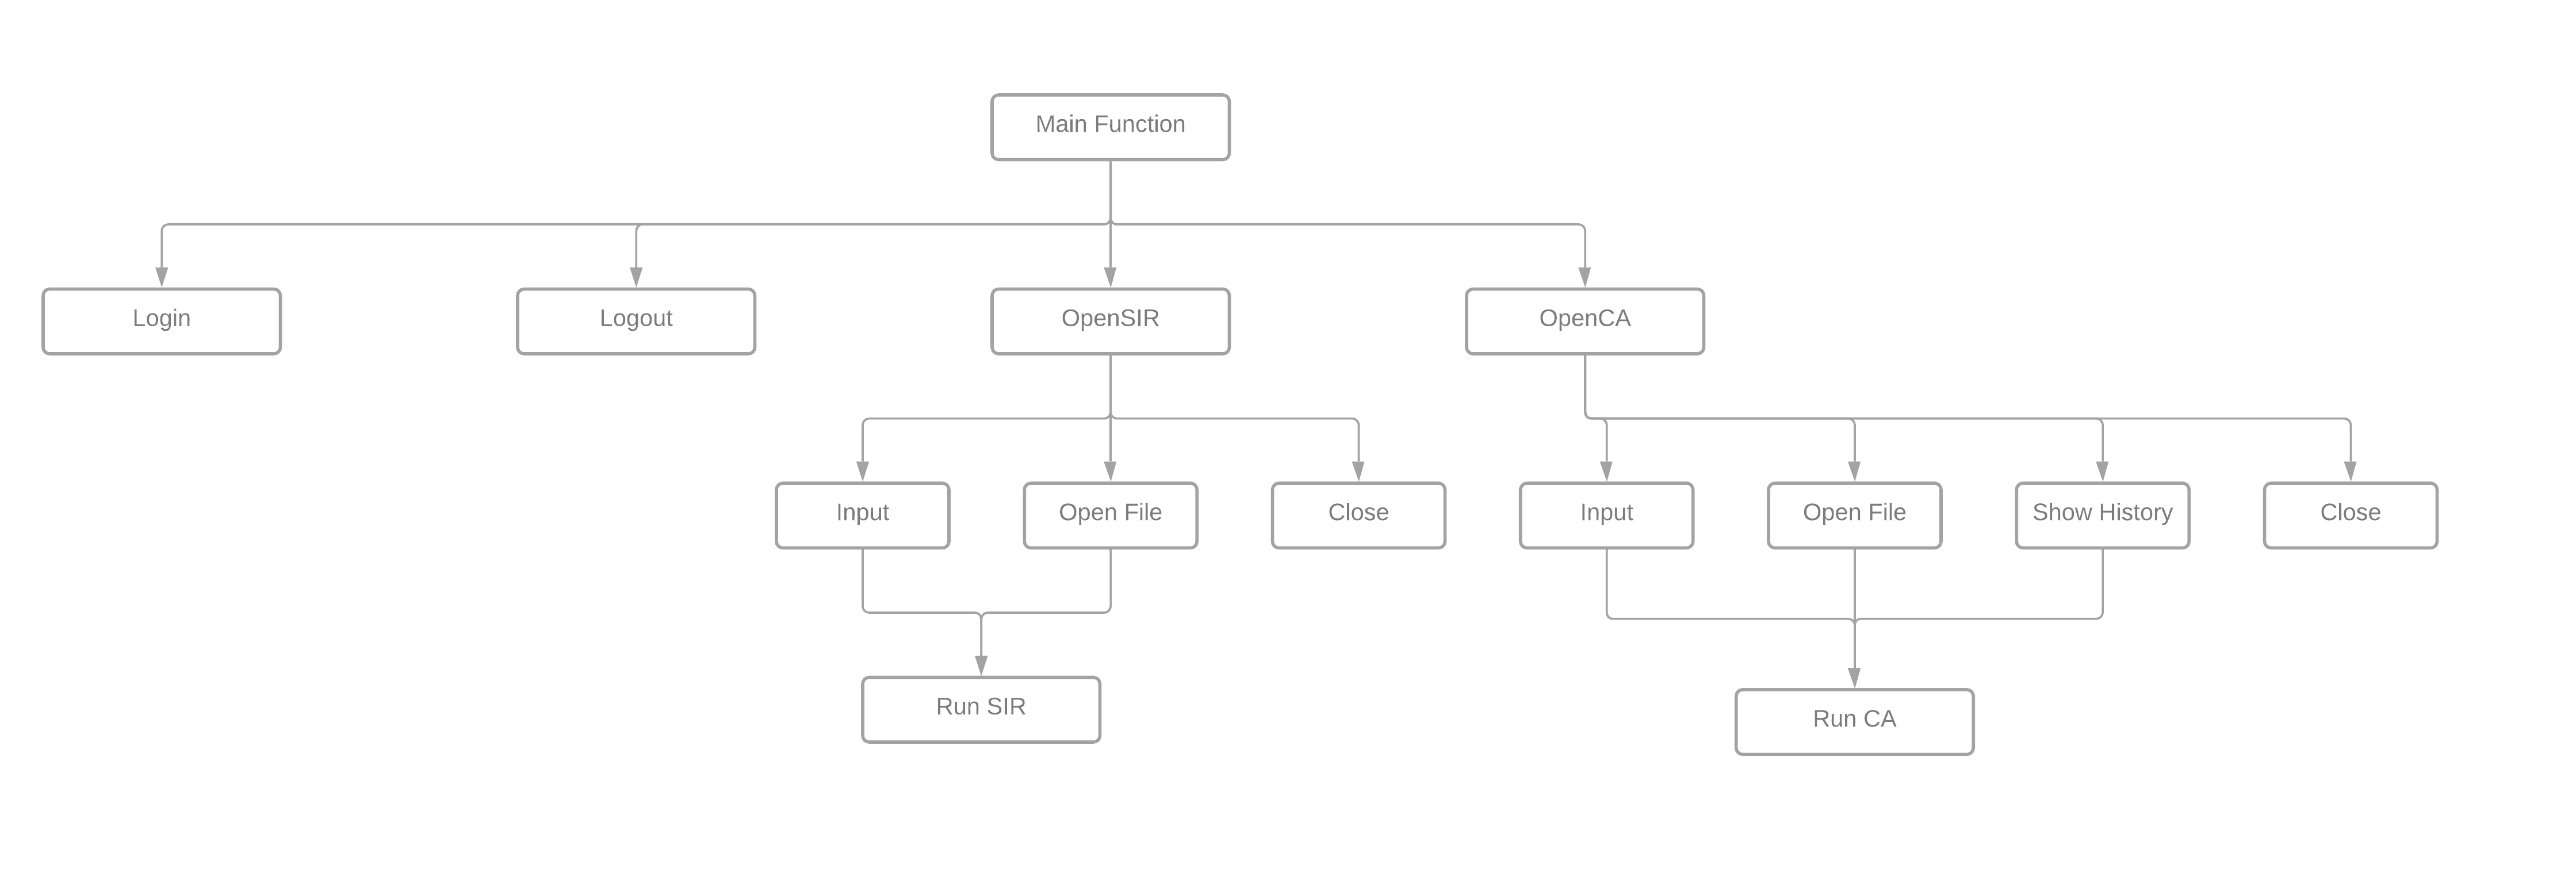
\includegraphics[height=5.43cm, width=\textwidth]{s_main_function.png}
\subsection{Main function flowchart}
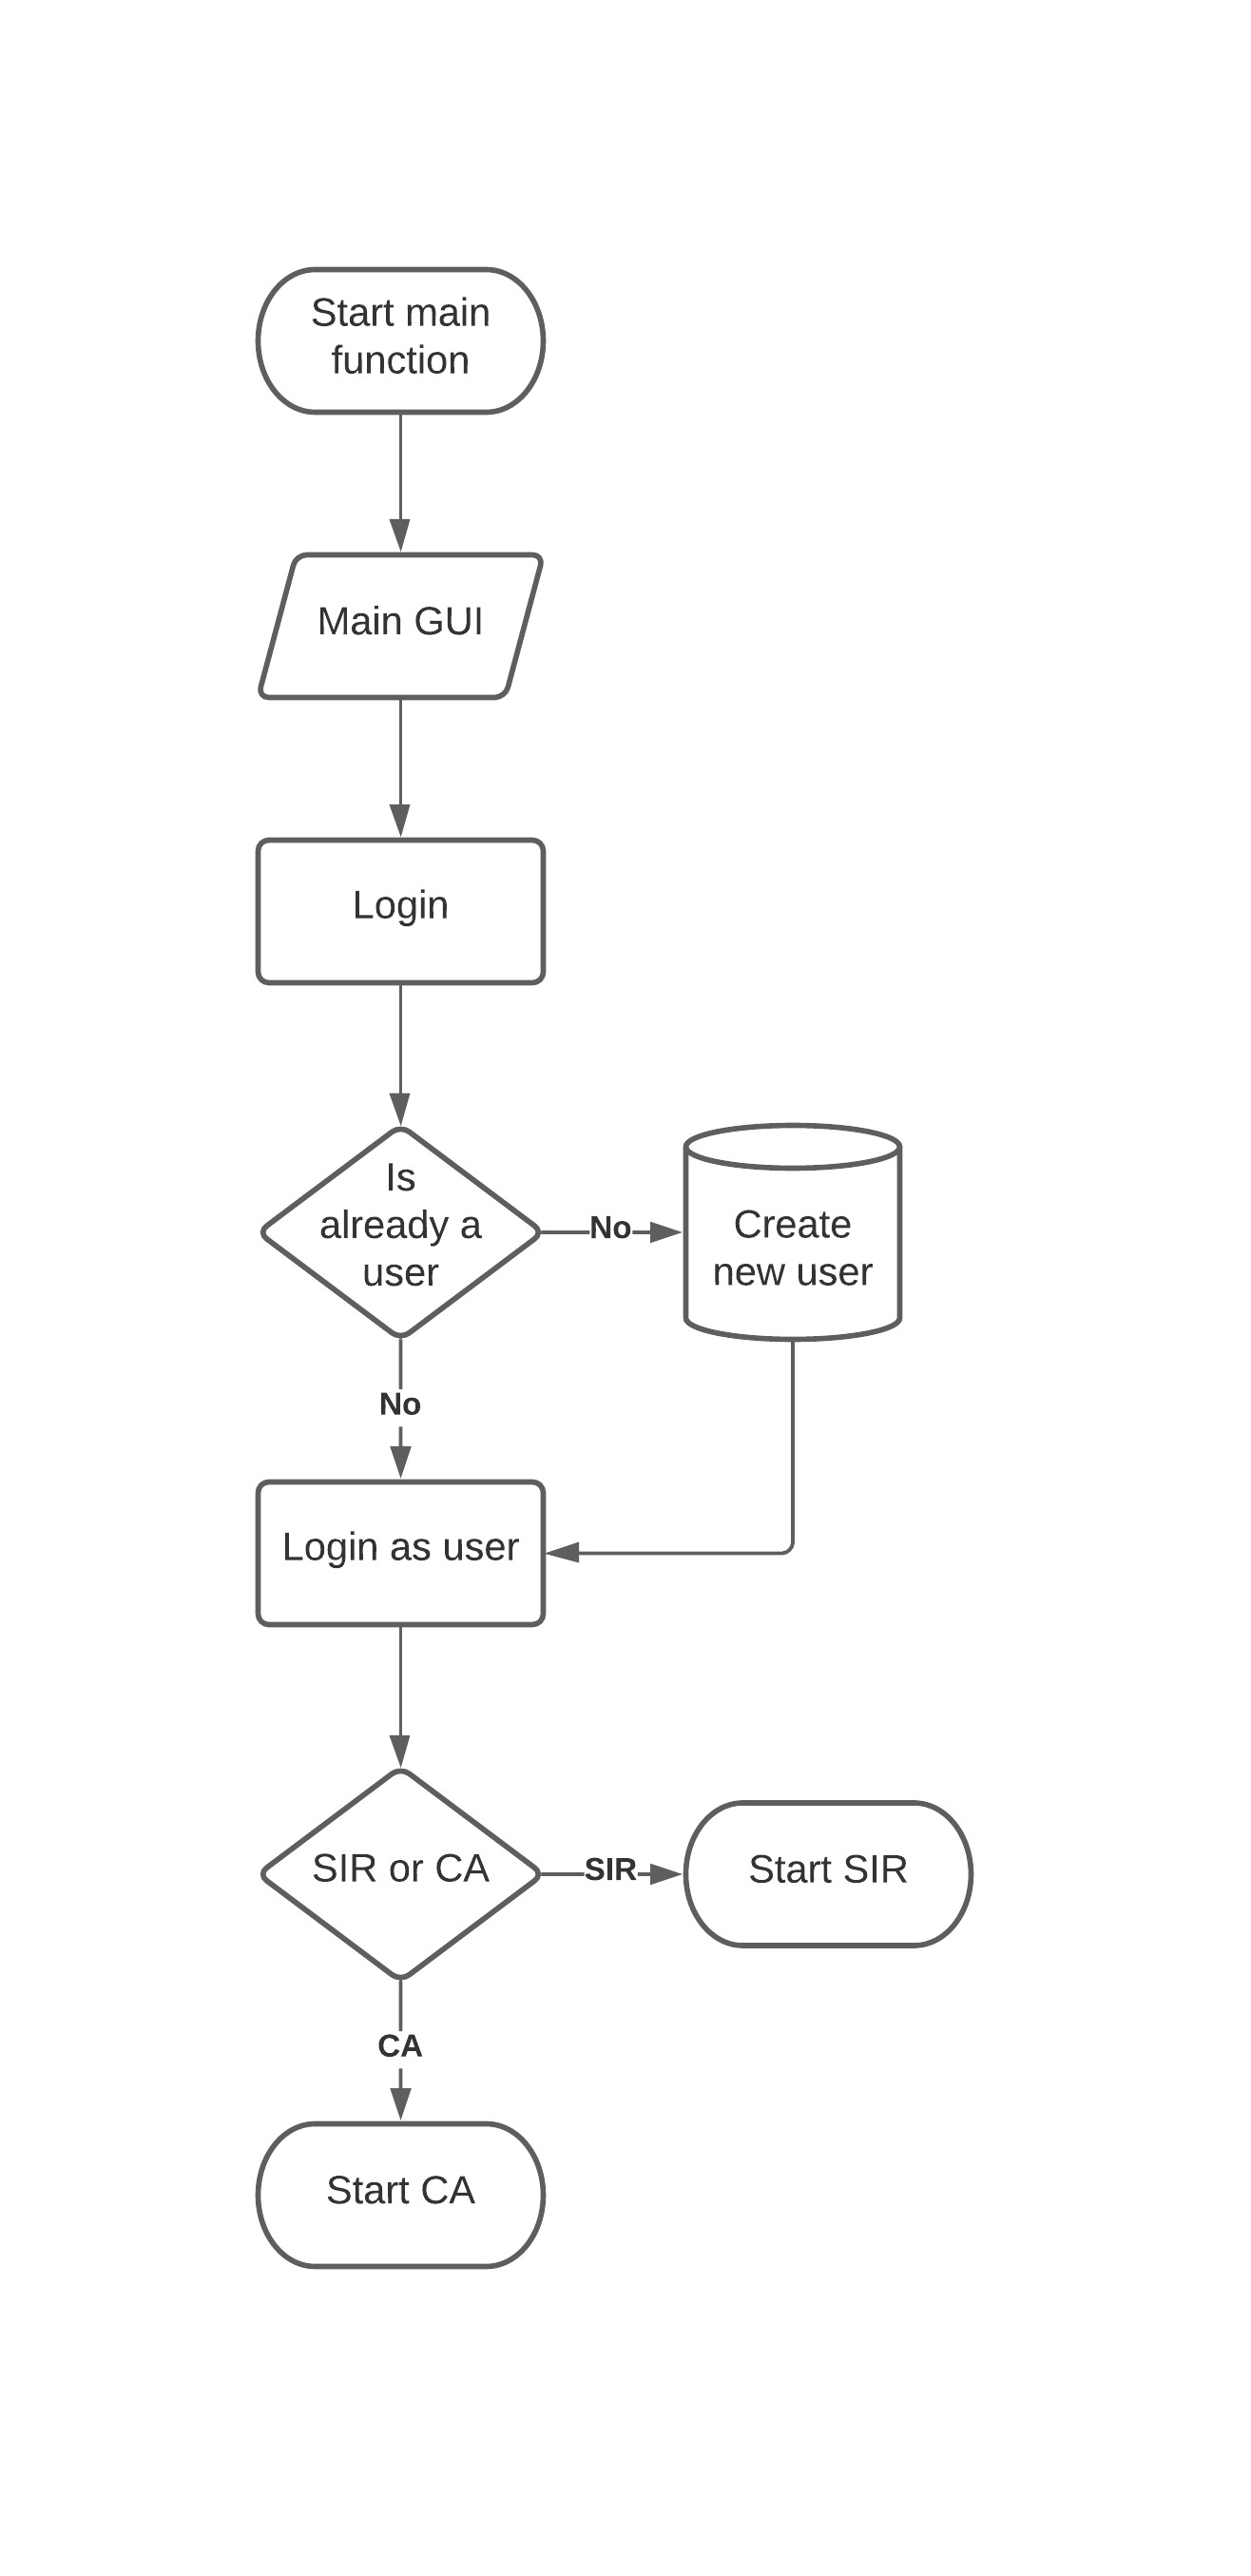
\includegraphics[height=15cm]{f_main.png}
\newpage
\subsection{Cellular automata structure diagram}
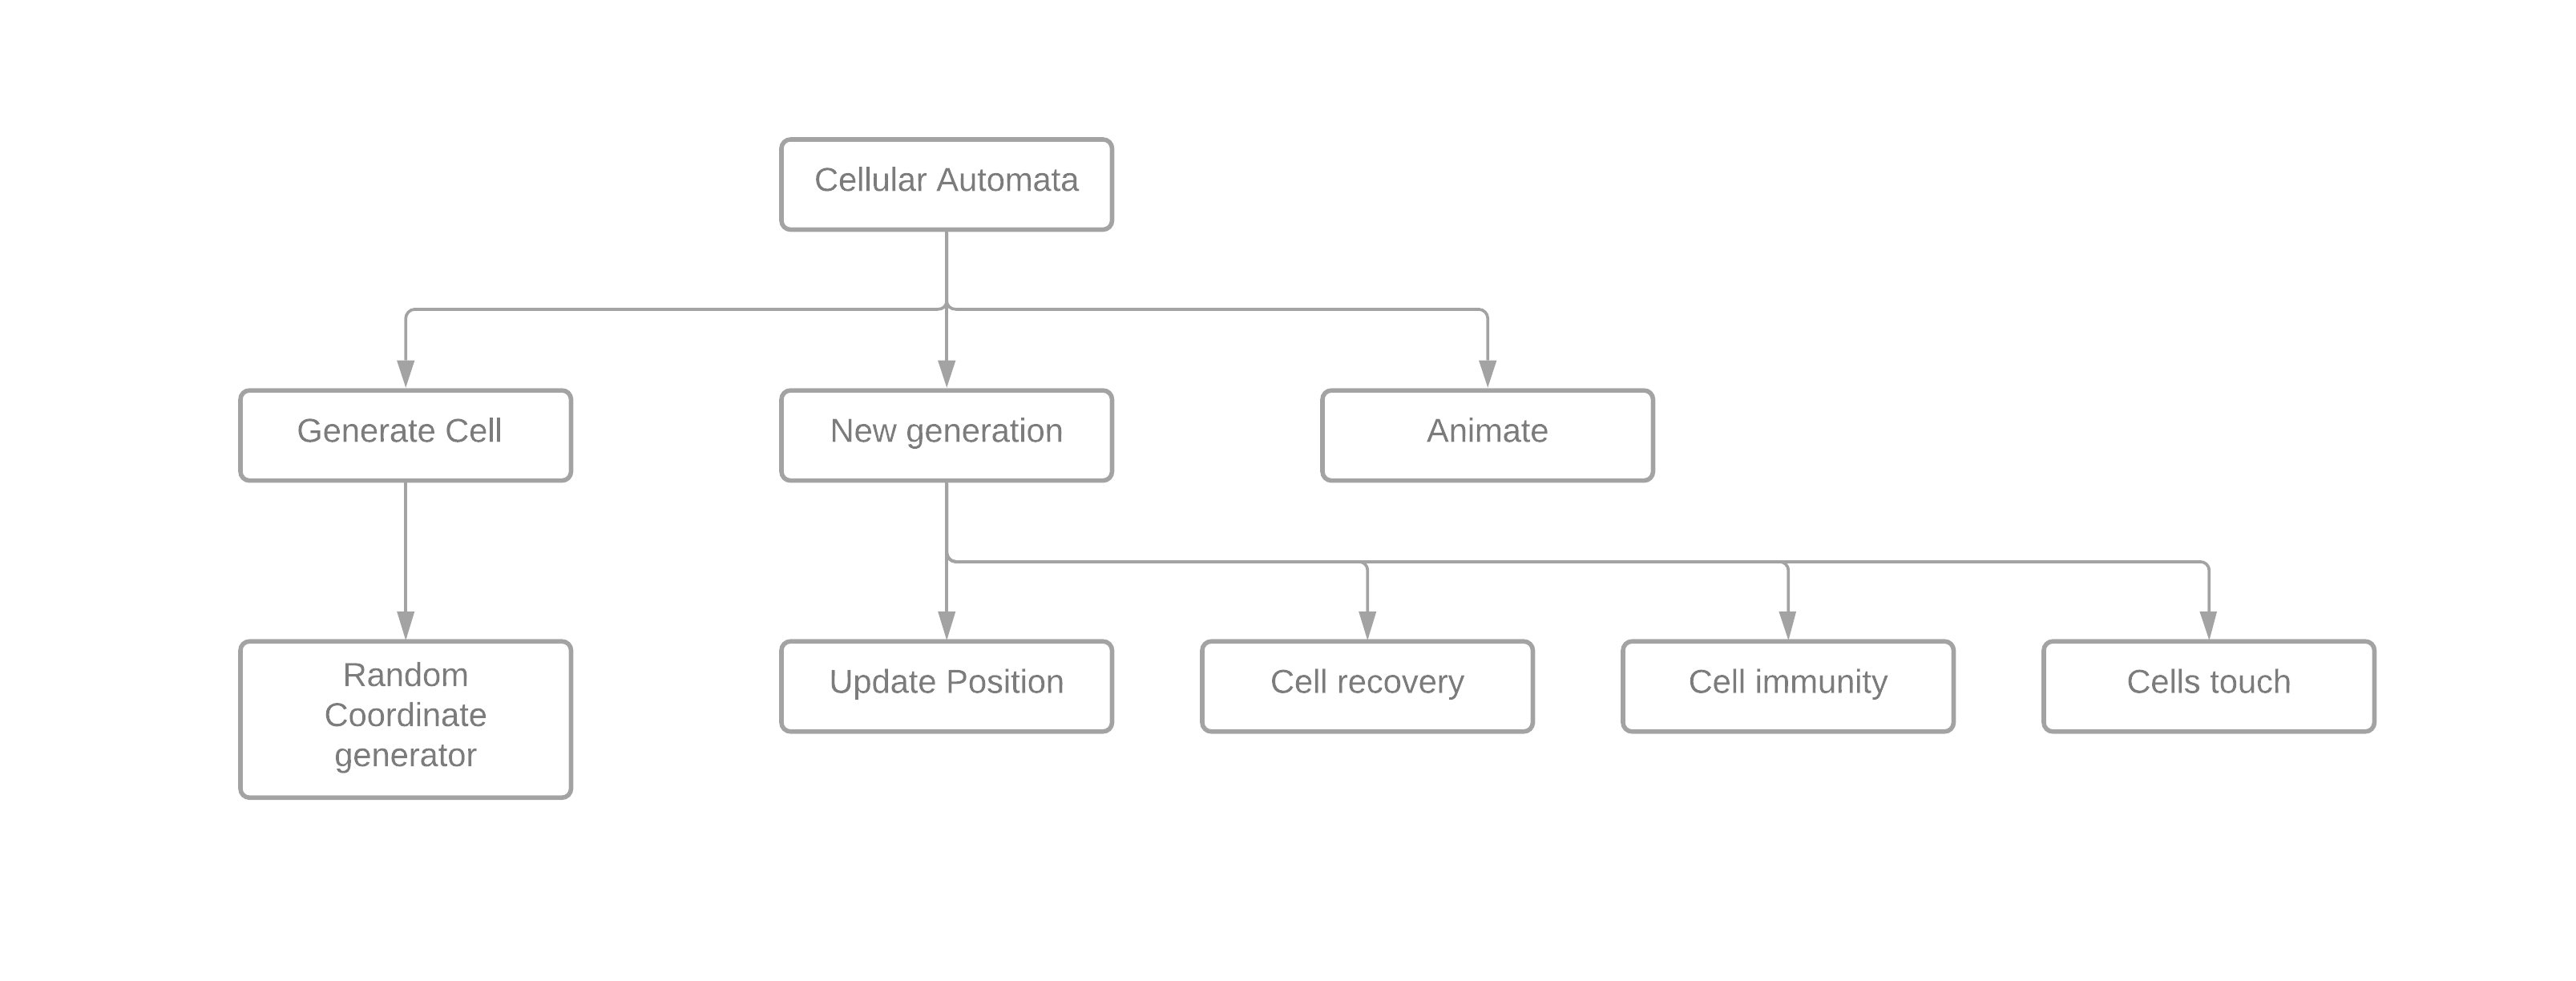
\includegraphics[height=5cm]{s_CA.png}
\subsection{Cellular automata flowchart}
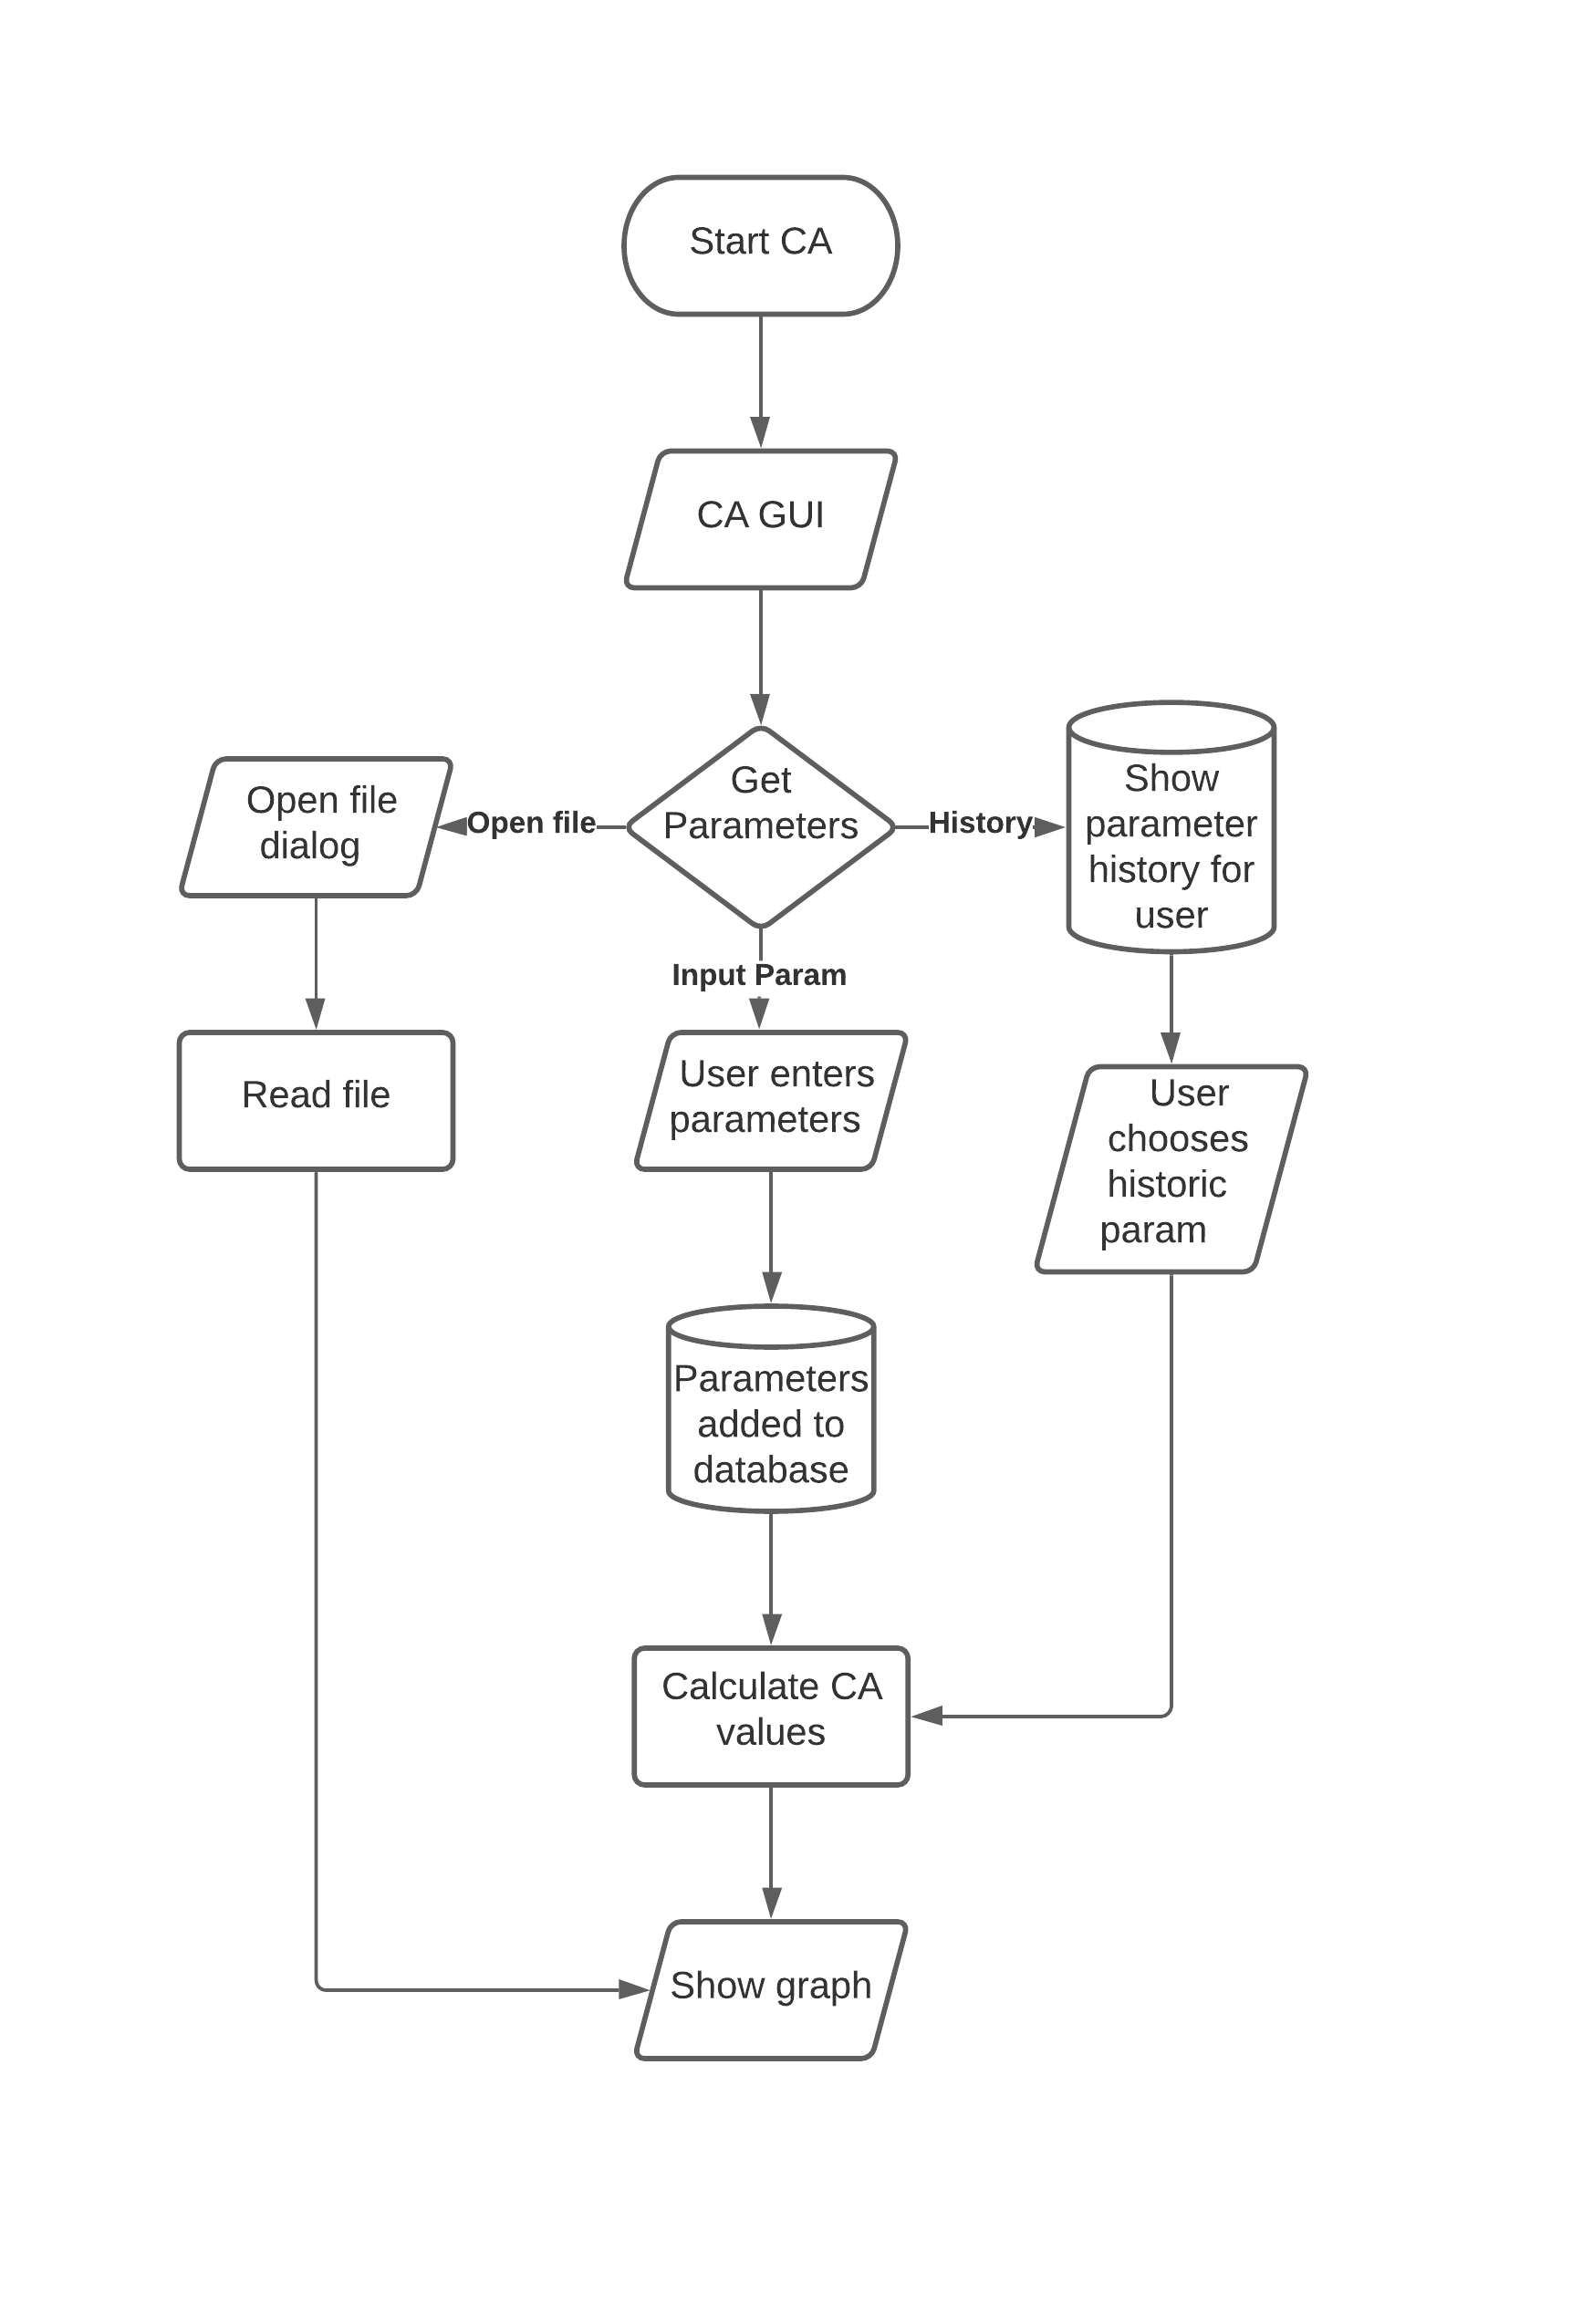
\includegraphics[height=15cm]{f_CA.png}
\newpage
\subsection{SIR Model structure diagram}
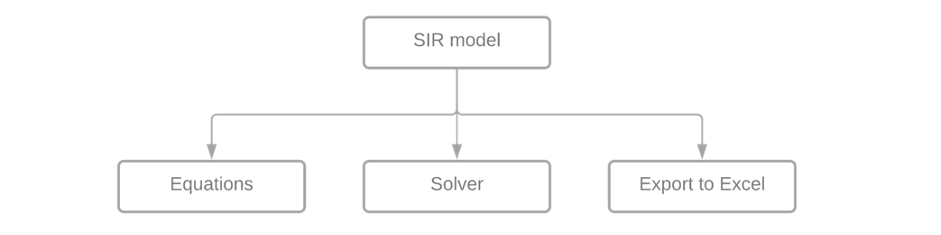
\includegraphics[height=3.6cm]{s_SIR.png}
\subsection{SIR model flowchart}
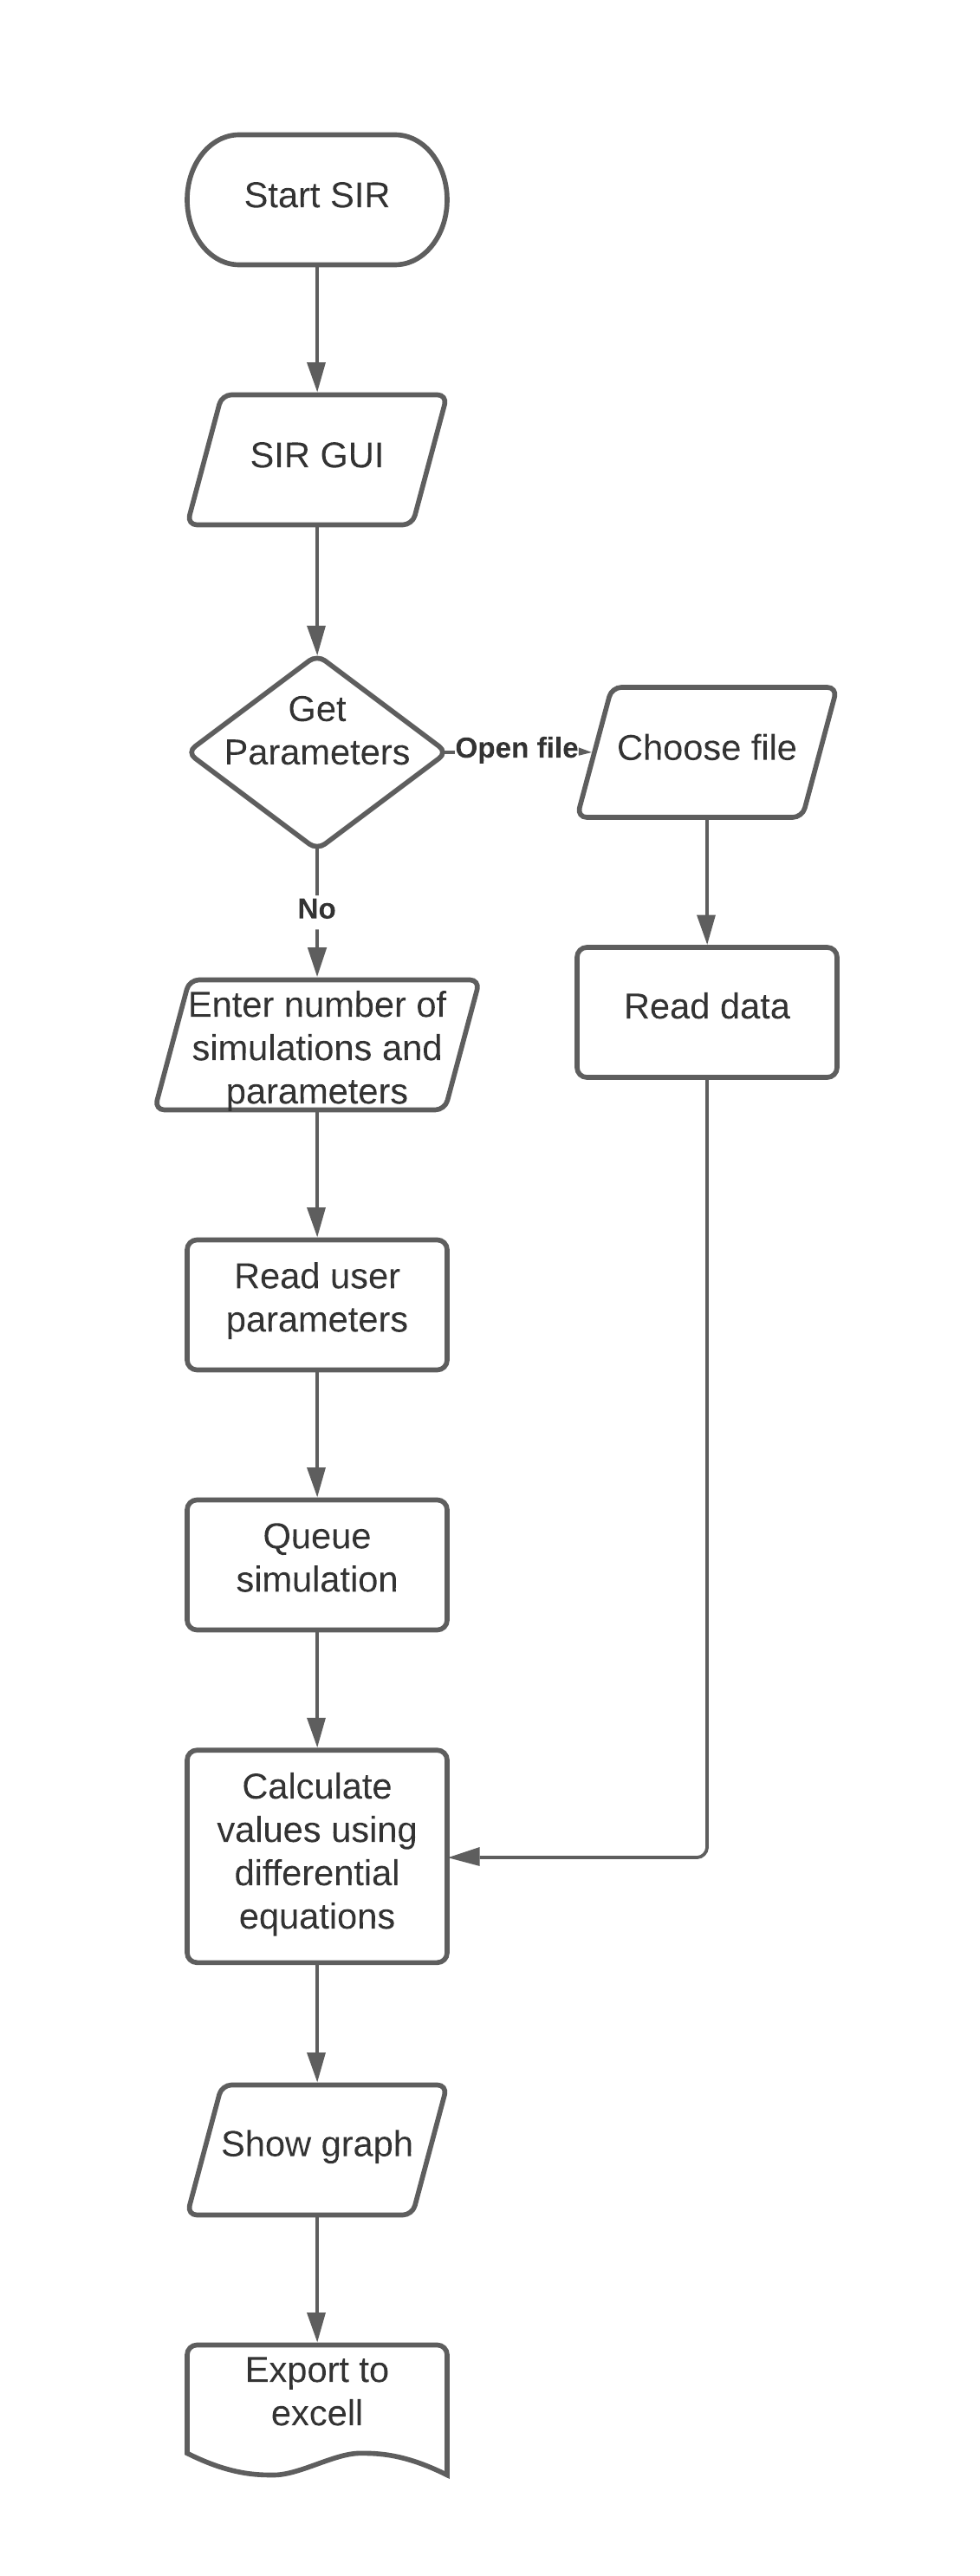
\includegraphics[height=17.3cm]{f_SIR.png}
\newpage
\subsection{Cellular automata and SIR model UML charts}
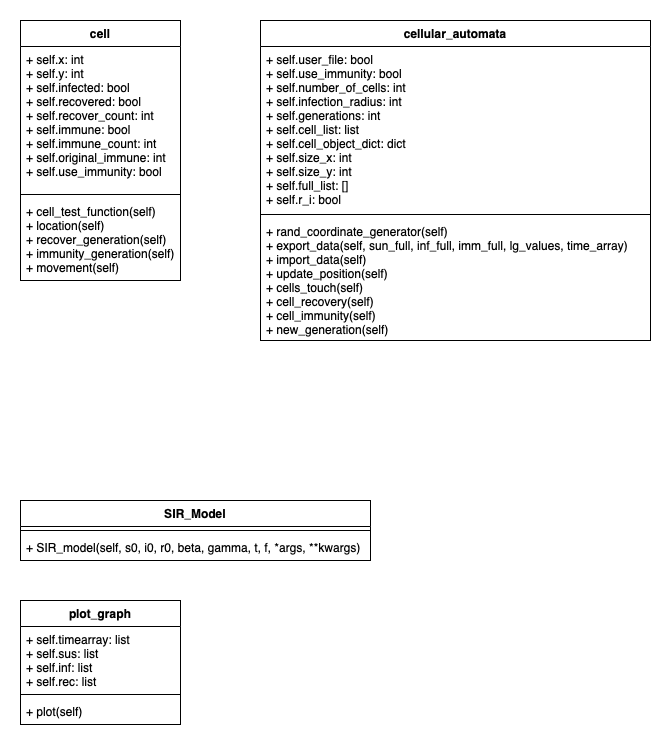
\includegraphics[width=\textwidth]{uml_ca_sir.png}
\subsection{SQL Entity relationship diagram}
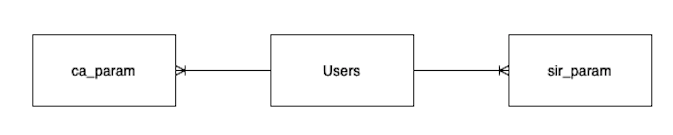
\includegraphics[width=\textwidth]{re_sql.png}
\subsection{SQL queries used}
\textbf{Creating a new table}
\begin{lstlisting}
CREATE TABLE users (username text PRIMARY KEY, see_all integer)

CREATE TABLE ca_param (
    user string,
    no_cells integer,
    generations integer,
    size_x integer,
    size_y integer,
    infection_radius integer,
    no_infected integer,
    recovered_can_be_infected integer,
    days_until_recovered integer,
    use_immunity integer,
    days_of_immunity integer    
    )

CREATE TABLE sir_param (
    user string,
    sus0 integer,
    inf0 integer,
    rec0 integer,
    beta integer,
    gamma integer,
    time integer
    )

INSERT INTO users VALUES (:username, :see_all), {'username': 'admin', 'see_all': 1}
\end{lstlisting}
This code sets up a clean database containing 3 tables, users, ca\_param and sir\_param. In the users table there are two columns, one containing the username and another containing a value to decide whether that user can see the history of all calculations performed and not just the calculations performed by that user. THIS WILL BE UPDATED. The ca\_param and sir\_param table contain columns to record the user doing the calculation and the parameters the user entered.

\textbf{Inserting a new user into the user table}
\begin{lstlisting}
INSERT OR IGNORE INTO users VALUES (:username, :see_all),{'username': in_user, 'see_all': 0}
\end{lstlisting}

\textbf{Entering parameters from the Cellular Automata model}
\begin{lstlisting}
INSERT INTO ca_param VALUES (
    :user, :no_cells, :generations, :size_x, :size_y,
    :infection_radius, :no_infected, :recovered_can_be_infected,
    :days_until_recovered, :use_immunity, :days_of_immunity),
    {'user': in_user, 'no_cells': up[0], 'generations': up[1], 'size_x': up[2], 'size_y': up[3],
        'infection_radius': up[4], 'no_infected': up[5], 'recovered_can_be_infected': up[6],
        'days_until_recovered': up[7], 'use_immunity': up[8], 'days_of_immunity': up[9]}
\end{lstlisting}
This query will be passed the user, in\_user, and a list of the parameters entered, up. This will be added into the ca\_param table.

\textbf{Entering parameters from the SIR model}
\begin{lstlisting}
INSERT INTO sir_param VALUES (:user, :sus0, :inf0, :rec0, :beta, :gamma, :time),{'user': in_user, 'sus0': up[0], 'inf0': up[1], 'rec0': up[2], 'beta': up[3], 'gamma': up[4], 'time': up[5]
    }
\end{lstlisting}
Similar to function above except for the SIR model

\textbf{Return history from Cellular Automata model}
\begin{lstlisting}
SELECT * FROM ca_param WHERE user=:curr_user, {'curr_user': in_user}
\end{lstlisting}

\textbf{Return history from SIR model}
\begin{lstlisting}
SELECT * FROM sir_param WHERE user=:curr_user, {'curr_user':in_user}
\end{lstlisting}



\subsection{UI design}
% \end{comment}

\newpage
\section{The code}

% \begin{comment}

\subsection{Main Function}
\begin{lstlisting}
# pylint: disable=unused-variable
import tkinter as tk
from tkinter import ttk
from scipy.integrate import odeint
import numpy as np
import matplotlib.pyplot as plt
import pandas as pd
import random
import time
from matplotlib.animation import FuncAnimation
import matplotlib
import csv
import json
from tkinter import filedialog
from tkinter import messagebox

import sub_SIR_model as my_sir
import sub_CA_model as my_ca
import sub_sql_functions as my_sql

current_user = "None"


class gui_Main_Window:
    """First window shown where user must login and can choose to simulate using either CA or openSIR
    """

    def __init__(self, master):
        self.master = master
        self.frame = ttk.Frame(master, padding=5)

        # self.lbl_name = ttk.Label(self.frame, text='This is the main page')
        self.e_user = ttk.Entry(self.frame)
        self.btn_login = ttk.Button(self.frame, text='Login', command=self.login)
        self.btn_SIR = ttk.Button(self.frame, text='SIR model', command=self.openSIR, state=tk.DISABLED)
        self.btn_CA = ttk.Button(self.frame, text='Cellular Automata', command=self.openCA, state=tk.DISABLED)

        self.frame.grid(row=0, column=0, sticky='nsew')

        # self.lbl_name.grid(column=1, row=0, columnspan=3, sticky='n')
        self.e_user.grid(column=1, row=0, sticky='n')
        self.btn_login.grid(column=2, row=0, sticky='n')
        self.btn_SIR.grid(column=1, row=1, columnspan=2, sticky='s')
        self.btn_CA.grid(column=1, row=2, columnspan=2, sticky='s')

        self.master.columnconfigure(0, weight=1)
        self.master.rowconfigure(0, weight=1)

        self.frame.columnconfigure(1, weight=1)
        self.frame.rowconfigure(1, weight=1)

        if current_user != "None":
            self.pers_login()

    def pers_login(self):
        self.btn_SIR['state'] = tk.NORMAL
        self.btn_CA['state'] = tk.NORMAL
        self.e_user.destroy()
        self.btn_login.destroy()
        self.lbl_name = ttk.Label(self.frame, text=f'Hello {current_user}')
        self.lbl_name.grid(column=1, row=0)
        self.btn_logout = ttk.Button(self.frame, text='logout', command=self.logout)
        self.btn_logout.grid(column=2, row=0)

    def openSIR(self):
        self.master.destroy()
        root2 = tk.Tk()
        root2.title('SIR Model')
        # root2.geometry('1400x900')
        new_window = gui_First_SIR_Window(root2)
        root2.mainloop()

    def openCA(self):
        self.master.destroy()
        root2 = tk.Tk()
        root2.title('CA Model')
        new_window = gui_First_CA_Window(root2)
        root2.mainloop()

    def login(self):
        """Gets username from user that was entered into username box, calls enter_username sql function with ti and assigns it to the current user global variable
        """
        username = str(self.e_user.get())
        my_sql.enter_username(username)
        global current_user
        current_user = username

        self.btn_SIR['state'] = tk.NORMAL
        self.btn_CA['state'] = tk.NORMAL
        self.e_user.destroy()
        self.btn_login.destroy()
        self.lbl_name = ttk.Label(self.frame, text=f'Hello {current_user}')
        self.lbl_name.grid(column=1, row=0)
        self.btn_logout = ttk.Button(self.frame, text='logout', command=self.logout)
        self.btn_logout.grid(column=2, row=0)

    def logout(self):
        print('logout')
        self.e_user = ttk.Entry(self.frame)
        self.btn_login = ttk.Button(self.frame, text='Login', command=self.login)
        self.e_user.grid(column=1, row=0, sticky='n')
        self.btn_login.grid(column=2, row=0, sticky='n')
        self.btn_SIR['state'] = tk.DISABLED
        self.btn_CA['state'] = tk.DISABLED
        current_user = "None"


class error:

    def __init__(self, err_type, message):
        tk.Tk().withdraw()
        title = err_type + " error"
        messagebox.showerror(title, message)


# ---------------------------------------

class gui_First_SIR_Window:
    """GUI where user can enter how many graphs they want to make, and whether they want to manually enter parameters, chose a file or use past parameters in history"""

    def __init__(self, master):
        self.master = master
        self.frame = ttk.Frame(master, padding=5)

        self.lbl_name = ttk.Label(self.frame, text='This is the SIR model')

        self.lbl_num_sim = ttk.Label(self.frame, text='Number of simulations')
        self.e_num_sim = ttk.Entry(self.frame)
        # self.num_sim.insert(0, 1)
        self.btn_open_file = ttk.Button(self.frame, text='Load File', command=self.open_file)
        self.btn_input_param = ttk.Button(self.frame, text='Enter Parameters', command=self.input)
        self.btn_history = ttk.Button(self.frame, text='Show History', command=self.show_history)
        self.btn_close = ttk.Button(self.frame, text='Close', command=self.close)

        self.frame.grid(row=0, column=0, sticky='nsew')

        self.lbl_name.grid(column=0, row=0, columnspan=2, sticky='n')
        self.lbl_num_sim.grid(column=0, row=1)
        self.e_num_sim.grid(column=1, row=1)
        # self.num_sim.grid(column=0, row=1)
        self.btn_open_file.grid(column=0, row=2)
        self.btn_input_param.grid(column=1, row=2)
        self.btn_history.grid(column=0, row=3)
        self.btn_close.grid(column=1, row=3, sticky='s')

        self.master.columnconfigure(0, weight=1)
        self.master.rowconfigure(0, weight=1)

        self.frame.columnconfigure(1, weight=1)
        self.frame.rowconfigure(1, weight=1)

    def close(self):
        self.master.destroy()
        main_win = tk.Tk()
        main_win.title('Main Window')
        new_window = gui_Main_Window(main_win)
        main_win.mainloop()

    def open_file(self):

        print("file dialog")
        filename = filedialog.askopenfilename()
        print(filename)
        df = pd.read_excel(filename)
        timearray = df['Time'].values.tolist()
        susceptible = df['S'].values.tolist()
        infected = df['I'].values.tolist()
        recovered = df['R'].values.tolist()

        self.master.destroy()

        plot = my_sir.plot_graph(timearray, susceptible, infected, recovered)
        plot.plot()

    def input(self):
        # print(type(self.e_num_sim.get()))
        try:
            int(self.e_num_sim.get())
            if 1 <= int(self.e_num_sim.get()) <= 10:
                self.number_of_simulations = int(self.e_num_sim.get())
                print(self.number_of_simulations)

                # self.number_of_simulations = 1
                self.master.destroy()
                root3 = tk.Tk()
                root3.title('Input Parameters')
                input_window = gui_SIR_Param(root3, self.number_of_simulations)
                root3.mainloop()
            else:
                err = error("Entry", "Please enter an integer between 1 and 10")
        except ValueError:
            err = error("Entry", "Please enter an integer between 1 and 10")



    def show_history(self):
        self.master.destroy()
        root3 = tk.Tk()
        root3.title('History')
        history_window = gui_SIR_history(root3)


class gui_SIR_Param:
    """Class for entering SIR parameters"""

    def __init__(self, master, num_sim):
        self.param_list = [[], [], [], [], []]
        self.counter = 0

        self.number_of_simulations = num_sim
        self.master = master
        self.frame = ttk.Frame(master, padding=5)
        self.frame.grid(row=0, column=0, sticky='nsew')

        # label variables
        self.lbl_name = ttk.Label(self.frame, text='Enter parameters for SIR model')
        self.s_name = ttk.Label(self.frame, text='Susceptible')
        self.i_name = ttk.Label(self.frame, text='Infected')
        self.r_name = ttk.Label(self.frame, text='Recovered')
        self.tr_name = ttk.Label(self.frame, text='Transmission rate')
        self.re_name = ttk.Label(self.frame, text='Recovery rate')
        self.btn_enter = ttk.Button(self.frame, text='Enter', command=self.enter_param)
        self.btn_close = ttk.Button(self.frame, text='Close', command=self.exit)

        # button variables
        self.e_s = ttk.Entry(self.frame)
        self.e_i = ttk.Entry(self.frame)
        self.e_r = ttk.Entry(self.frame)
        self.e_tr = ttk.Entry(self.frame)
        self.e_re = ttk.Entry(self.frame)

        # gridding label variables
        self.lbl_name.grid(column=0, row=0, columnspan=2, sticky='n')
        self.s_name.grid(column=0, row=1, sticky='w')
        self.i_name.grid(column=0, row=2, sticky='w')
        self.r_name.grid(column=0, row=3, sticky='w')
        self.tr_name.grid(column=0, row=4, sticky='w')
        self.re_name.grid(column=0, row=5, sticky='w')

        self.e_s.grid(column=1, row=1, sticky='w')
        self.e_i.grid(column=1, row=2, sticky='w')
        self.e_r.grid(column=1, row=3, sticky='w')
        self.e_tr.grid(column=1, row=4, sticky='w')
        self.e_re.grid(column=1, row=5, sticky='w')

        self.btn_enter.grid(column=1, row=6, columnspan=1)
        self.btn_close.grid(column=0, row=6, columnspan=1)

        self.master.columnconfigure(0, weight=1)
        self.master.rowconfigure(0, weight=1)

        # weight elements for resizing
        self.frame.columnconfigure(0, weight=1)
        self.frame.rowconfigure(0, weight=1)
        self.frame.rowconfigure(1, weight=1)
        self.frame.rowconfigure(2, weight=1)
        self.frame.rowconfigure(3, weight=1)
        self.frame.rowconfigure(4, weight=1)
        self.frame.rowconfigure(5, weight=1)
        self.frame.rowconfigure(6, weight=1)

    def enter_param(self):
        self.counter += 1

        self.param_list[0].append(float(self.e_s.get()))
        self.param_list[1].append(float(self.e_i.get()))
        self.param_list[2].append(float(self.e_r.get()))
        self.param_list[3].append(float(self.e_tr.get()))
        self.param_list[4].append(float(self.e_re.get()))

        self.e_s.delete(0, 'end')
        self.e_i.delete(0, 'end')
        self.e_r.delete(0, 'end')
        self.e_tr.delete(0, 'end')
        self.e_re.delete(0, 'end')

        if self.counter == self.number_of_simulations:
            self.submit_param()
            self.counter = 0

    def submit_param(self):
        """Creates queue object from my_sir function and calls the run simulation function
        """
        # print(self.param_list)
        self.master.destroy()

        pass1 = True
        for sub_list in self.param_list:
            for value in sub_list:
                if value < 0:
                    pass1 = False
                    err = error("Value", "Negative numbers cannot be used for any of these inputs")

        if not pass1:
            root3 = tk.Tk()
            root3.title('Input Parameters')
            input_window = gui_SIR_Param(root3, self.number_of_simulations)
            root3.mainloop()
        else:
            queue = my_sir.QueueSimulation(self.number_of_simulations, self.param_list[0], self.param_list[1],
                                           self.param_list[2],
                                           self.param_list[3], self.param_list[4],
                                           1000, current_user)

            queue.run_simulation()

    def exit(self):
        self.master.destroy()
        sir_win = tk.Tk()
        sir_win.title('SIR')
        sir_main = gui_First_SIR_Window(sir_win)


class gui_SIR_history:

    def __init__(self, master):
        self.master = master
        self.frame = ttk.Frame(master, padding=5)
        self.frame.grid(row=0, column=0, sticky='nsew')
        self.user_history = my_sql.sir_return_history(current_user)  # user_history is a list of tuples
        print(self.user_history)
        # print(self.user_history[0][1:])

        self.lb_history = tk.Listbox(self.frame, width=50)
        for i in range(len(self.user_history)):
            to_insert = str(i) + "  " + str(self.user_history[i][1:])
            self.lb_history.insert(i, to_insert)

        self.lbl_title = ttk.Label(self.frame, text=f"History of {current_user}")
        self.btn_exit = ttk.Button(self.frame, text="Exit", command=self.exit)
        self.lbl_text = ttk.Label(self.frame, text="Enter number to simulate with same parameters")
        self.e_sim_num = ttk.Entry(self.frame)
        self.btn_use = ttk.Button(self.frame, text="Use values", command=self.use)

        self.lbl_title.grid(column=1, row=1, columnspan=3)
        self.lbl_text.grid(column=1, row=2, columnspan=3)
        self.lb_history.grid(column=1, row=3)
        self.e_sim_num.grid(column=2, row=3)
        self.btn_use.grid(column=3, row=3)
        self.btn_exit.grid(column=2, row=4, columnspan=2)

    def exit(self):
        self.master.destroy()
        sir_win = tk.Tk()
        sir_win.title('SIR')
        sir_main = gui_First_SIR_Window(sir_win)

    def use(self):
        """User enter number and set of parameters are retrieved from the database"""
        sim_number = int(self.e_sim_num.get())
        sim_param = list(self.user_history[sim_number][1:])
        print(sim_param)

        queue = my_sir.QueueSimulation(1, [sim_param[0]], [sim_param[1]], [sim_param[2]], [sim_param[3]],
                                       [sim_param[4]], sim_param[5], current_user)

        queue.run_simulation()


# ---------------------------------------

class gui_First_CA_Window:
    """GUI window where user can enter parameters manually, load file generated or show history of previously used parameters and choose one for the ceccular automata model
    """

    def __init__(self, master):
        self.master = master
        self.frame = ttk.Frame(master, padding=5)

        self.lbl_name = ttk.Label(self.frame, text='This is the Cellular Automata model')
        # self.num_sim = ttk.Entry(self.frame)
        # self.num_sim.insert(0, 1)
        self.btn_open_file = ttk.Button(self.frame, text='Load File', command=self.open_file)
        self.btn_input_param = ttk.Button(self.frame, text='Enter Parameters', command=self.input)
        self.btn_show_history = ttk.Button(self.frame, text='History', command=self.show_history)
        self.btn_close = ttk.Button(self.frame, text='Close', command=self.close)

        self.frame.grid(row=0, column=0, sticky='nsew')

        self.lbl_name.grid(column=0, row=0, columnspan=2, sticky='n')
        # self.num_sim.grid(column=0, row=1)
        self.btn_open_file.grid(column=0, row=1)
        self.btn_input_param.grid(column=1, row=1)
        self.btn_show_history.grid(column=0, row=2)
        self.btn_close.grid(column=1, row=2, sticky='s')

        self.master.columnconfigure(0, weight=1)
        self.master.rowconfigure(0, weight=1)

        self.frame.columnconfigure(1, weight=1)
        self.frame.rowconfigure(1, weight=1)

    def open_file(self):
        # enter file stuff
        print("Opening file dialog")
        file = filedialog.askopenfile(mode="r")
        lines = [line.rstrip('\n') for line in file]
        file.close()

        if lines[-1] == "":
            del lines[-1]

        # result = [json.loads(item) for item in lines]
        self.master.destroy()

        ca = my_ca.cellular_automata(0, 0, 0, 0, 0, 0, False, 0, False, 0, True, lines)
        ca.new_generation()
        self.master.destroy()

    def input(self):
        # manual user input
        self.master.destroy()
        root3 = tk.Tk()
        root3.title('Input Parameters')
        input_window = gui_CA_Param(root3)

    def show_history(self):
        self.master.destroy()
        root3 = tk.Tk()
        root3.title('History')
        history_window = gui_CA_history(root3)

    def close(self):
        self.master.destroy()
        main_win = tk.Tk()
        main_win.title('Main Window')
        new_window = gui_Main_Window(main_win)
        main_win.mainloop()


class gui_CA_Param:
    """GUI interface for inputting cellular automata parameters manually
    Need to make some entry boxes dependent on checkboxes
    """

    def __init__(self, master):
        self.master = master
        self.frame = ttk.Frame(master, padding=5)
        self.frame.grid(row=0, column=0, sticky='nsew')

        # label variables
        self.l_lbl_name = ttk.Label(self.frame, text='Enter parameters for CA model')
        self.l_no_cells = ttk.Label(self.frame, text='Number of cells')
        self.l_gen = ttk.Label(self.frame, text='Generations')
        self.l_size_x = ttk.Label(self.frame, text='Size x')
        self.l_size_y = ttk.Label(self.frame, text='Size y')
        self.l_inf_rad = ttk.Label(self.frame, text='Infection radius')
        self.l_no_inf = ttk.Label(self.frame, text='Number of infected')
        self.l_r_i = ttk.Label(self.frame, text='Recovered can be infected?')
        self.l_d_r = ttk.Label(self.frame, text='Days until recovery')
        self.l_use_imm = ttk.Label(self.frame, text='Use immunity')
        self.l_d_i = ttk.Label(self.frame, text='Days of immunity')

        # bool values for checkbuttons
        self.b_r_i = tk.BooleanVar()
        self.b_u_i = tk.BooleanVar()

        # entry and checkbutton variables
        self.e_no_cells = ttk.Entry(self.frame)
        self.e_gen = ttk.Entry(self.frame)
        self.e_size_x = ttk.Entry(self.frame)
        self.e_size_y = ttk.Entry(self.frame)
        self.e_inf_rad = ttk.Entry(self.frame)
        self.e_no_inf = ttk.Entry(self.frame)
        self.cb_r_i = ttk.Checkbutton(self.frame, variable=self.b_r_i)
        self.e_d_r = ttk.Entry(self.frame)
        self.cb_use_imm = ttk.Checkbutton(self.frame, variable=self.b_u_i)
        self.e_d_i = ttk.Entry(self.frame)

        self.btn_enter = ttk.Button(self.frame, text='Enter', command=self.enter_param)
        self.btn_close = ttk.Button(self.frame, text='Close', command=self.close)

        # grid label variables
        self.l_lbl_name.grid(column=0, row=0, columnspan=2, sticky='n')
        self.l_no_cells.grid(column=0, row=1, sticky='w')
        self.l_gen.grid(column=0, row=2, sticky='w')
        self.l_size_x.grid(column=0, row=3, sticky='w')
        self.l_size_y.grid(column=0, row=4, sticky='w')
        self.l_inf_rad.grid(column=0, row=5, sticky='w')
        self.l_no_inf.grid(column=0, row=6, sticky='w')
        self.l_r_i.grid(column=0, row=7, sticky='w')
        self.l_d_r.grid(column=2, row=7, sticky='w')
        self.l_use_imm.grid(column=0, row=8, sticky='w')
        self.l_d_i.grid(column=2, row=8, sticky='w')

        # grid entry variables
        self.e_no_cells.grid(column=2, row=1, sticky='w')
        self.e_gen.grid(column=2, row=2, sticky='w')
        self.e_size_x.grid(column=2, row=3, sticky='w')
        self.e_size_y.grid(column=2, row=4, sticky='w')
        self.e_inf_rad.grid(column=2, row=5, sticky='w')
        self.e_no_inf.grid(column=2, row=6, sticky='w')
        self.cb_r_i.grid(column=1, row=7, sticky='w')
        self.e_d_r.grid(column=3, row=7, sticky='w')
        self.cb_use_imm.grid(column=1, row=8, sticky='w')
        self.e_d_i.grid(column=3, row=8, sticky='w')

        self.btn_enter.grid(column=0, row=9, columnspan=2, sticky='s')
        self.btn_close.grid(column=2, row=9, columnspan=2, sticky='s')

        # grid main column and tow
        self.master.columnconfigure(0, weight=1)
        self.master.rowconfigure(0, weight=1)

        # weight elements for resizing
        self.frame.columnconfigure(0, weight=1)
        self.frame.rowconfigure(0, weight=1)
        self.frame.rowconfigure(1, weight=1)
        self.frame.rowconfigure(2, weight=1)
        self.frame.rowconfigure(3, weight=1)
        self.frame.rowconfigure(4, weight=1)
        self.frame.rowconfigure(5, weight=1)
        self.frame.rowconfigure(6, weight=1)

    def enter_param(self):
        """Gets values that were input, creates a cellular automata object and calls the new_generation function to start the cellular automata function
        """
        # should call CA function in this
        no_cells = int(self.e_no_cells.get())
        generations = int(self.e_gen.get())
        size_x = int(self.e_size_x.get())
        size_y = int(self.e_size_y.get())
        inf_rad = int(self.e_inf_rad.get())
        no_inf = int(self.e_no_inf.get())
        rec_inf = self.b_r_i.get()
        days_rec = int(self.e_d_r.get())
        use_imm = self.b_u_i.get()
        days_imm = int(self.e_d_i.get())

        self.master.destroy()
        # print(rec_inf)
        # print(use_imm)

        arguments = [no_cells, generations, size_x, size_y, inf_rad, no_inf, rec_inf, days_rec, use_imm,
                     days_imm, False]

        my_sql.ca_enter_param(current_user, arguments)

        # ca = my_ca.cellular_automata(no_cells, generations, size_x, size_y, inf_rad, no_inf, rec_inf, days_rec, use_imm,
        #                              days_imm, False)
        ca = my_ca.cellular_automata(*arguments)  # arguments sent as separate parameters

        ca.new_generation()

    def close(self):
        self.master.destroy()
        main_ca = tk.Tk()
        main_ca.title('CA')
        new_window = gui_First_CA_Window(main_ca)
        main_ca.mainloop()


class gui_CA_history:

    def __init__(self, master):
        self.master = master
        self.frame = ttk.Frame(master, padding=5)
        self.frame.grid(row=0, column=0, sticky='nsew')
        self.user_history = my_sql.ca_return_history(current_user)  # user_history is a list of tuples
        print(self.user_history)
        # print(self.user_history[0][1:])

        self.lb_history = tk.Listbox(self.frame, width=50)
        for i in range(len(self.user_history)):
            to_insert = str(i) + "  " + str(self.user_history[i][1:])
            self.lb_history.insert(i, to_insert)

        self.lbl_title = ttk.Label(self.frame, text=f"History of {current_user}")
        self.btn_exit = ttk.Button(self.frame, text="Exit", command=self.exit)
        self.lbl_text = ttk.Label(self.frame, text="Enter number to simulate with same parameters")
        self.e_sim_num = ttk.Entry(self.frame)
        self.btn_use = ttk.Button(self.frame, text="Use values", command=self.use)

        self.lbl_title.grid(column=1, row=1, columnspan=3)
        self.lbl_text.grid(column=1, row=2, columnspan=3)
        self.lb_history.grid(column=1, row=3)
        self.e_sim_num.grid(column=2, row=3)
        self.btn_use.grid(column=3, row=3)
        self.btn_exit.grid(column=2, row=4, columnspan=2)

    def exit(self):
        self.master.destroy()
        main_ca = tk.Tk()
        main_ca.title('CA')
        new_window = gui_First_CA_Window(main_ca)
        main_ca.mainloop()

    def use(self):
        """User enter number and set of parameters are retrieved from the database"""
        sim_number = int(self.e_sim_num.get())
        sim_param = list(self.user_history[sim_number][1:])
        print(sim_param)
        sim_param.append(False)
        ca = my_ca.cellular_automata(*sim_param)
        ca.new_generation()


# ---------------------------------------


root = tk.Tk()
root.title('Main Window')
root.geometry("300x100")

window = gui_Main_Window(root)
# window = gui_First_CA_Window(root)
current_user = "zebedee"

root.mainloop()

\end{lstlisting}

\subsection{SIR Model Function}
\begin{lstlisting}
    import matplotlib.pyplot as plt
    import pandas as pd
    import sub_sql_functions as my_sql
    
    
    class QueueSimulation:
    
        def __init__(self, n, s_list, i_list, r_list, b_list, g_list, t, current_user):
            self.n = n  # number of simulations to be run
            self.parameters = []
            for i in range(n):
                self.parameters.append([s_list[i], i_list[i], r_list[i], b_list[i], g_list[i], t, i + 1])
                my_sql.sir_enter_param(current_user, [s_list[i], i_list[i], r_list[i], b_list[i], g_list[i], t])
            print(self.parameters)
    
        def run_simulation(self):
            sir_model = SIR_model()
            for i in range(self.n):
                sir_model.SIR_model(*self.parameters[i])
            plt.show()
    
    
    class SIR_model:
    
        def __init__(self):
            pass
    
        def SIR_model(self, s0, i0, r0, beta, gamma, t, f, *args, **kwargs):
            """
            :param s0: number of susceptible people
            :param i0: number of infected people
            :param r0: number of recovered people
            :param beta: transmission rate of an individual
            :param gamma: recovery rate of an individual
            :param t: how long the simulation should run for
            :param f: how many graphs should be calculated simultaneously
            """
    
            plt.figure(f)  # names the graph
            N = s0 + i0 + r0  # total population
    
            timearray = list(range(1, int(t)))  # creates time array
    
            def eqns(param):
                # e = random.uniform(0, 1)
                e = 0
                S, I, R = param
                dsdt = (-(beta * S * I) / N) + (e * R)  # rate of change of susceptible individuals
                didt = ((beta * S * I) / N) - gamma * I  # rate of change of infected individuals
                drdt = (gamma * I) - (e * R)  # rate of change of recovered individuals
                return dsdt, didt, drdt
    
            def solver():  # solves differential equations in eqns
                param = (s0, i0, r0)
                solver_result = [[], [], []]
                for time in timearray:
                    eqns_results = eqns(param)
                    x, y, z = (param[0] + eqns_results[0]), (param[1] + eqns_results[1]), (param[2] + eqns_results[2])
                    solver_result[0].append(x)
                    solver_result[1].append(y)
                    solver_result[2].append(z)
                    param = (x, y, z)
                return solver_result
    
            solver_result = solver()
    
            # print(solver_result)
    
            def export_to_excel():  # exports calculated results to excel
                data = {'Time': timearray,
                        'S': solver_result[0],
                        'I': solver_result[1],
                        'R': solver_result[2]}
    
                df = pd.DataFrame(data, columns=['Time', 'S', 'I', 'R'])
                name = "output" + str(f) + ".xls"
                df.to_excel(name, sheet_name='output')
    
            export_to_excel()
            plt.plot(timearray, solver_result[0], label="S(t)")
            plt.plot(timearray, solver_result[1], label="I(t)")
            plt.plot(timearray, solver_result[2], label="R(t)")
    
    
    class plot_graph:
    
        def __init__(self, ta, s, i, r):
            # deconstruct file here
            self.timearray = ta
            self.sus = s
            self.inf = i
            self.rec = r
    
        def plot(self):
            plt.plot(self.timearray, self.sus, label="S(t)")
            plt.plot(self.timearray, self.inf, label="I(t)")
            plt.plot(self.timearray, self.rec, label="R(t)")
            plt.show()
    
\end{lstlisting}

\subsection{CA Function}
\begin{lstlisting}
    # pylint: disable=unused-variable
    # pylint: enable=too-many-lines
    
    import matplotlib.pyplot as plt
    import random
    from matplotlib.animation import FuncAnimation
    import json
    
    
    class cell:
        """Each cell will be a class instance of this class"""
    
        def __init__(self, x, y, infected, d_r, d_i, u_i):
            self.x = x
            self.y = y
            self.infected = infected
            self.recovered = False
            self.recover_count = d_r  # default - can be changed - time until infected cell recovers
            self.immune = False
            self.immune_count = d_i
            self.original_immune = d_i
            self.use_immunity = u_i
            # self.infection_rate = i
    
        def cell_test_function(self):
            return self.x, self.y, self.infected
    
        def location(self):
            # print(self.x, self.y)
            return self.x, self.y
    
        def recover_generation(self):
            self.recover_count -= 1
            if self.recover_count <= 0:
                self.recovered = True
                self.infected = False
                self.recover_count = 10
                if self.use_immunity:
                    self.immune = True
    
        def immunity_generation(self):
            if self.immune:
                self.immune_count -= 1
                if self.immune_count <= 0:
                    self.immune = False
                    self.immune_count = self.original_immune
    
        def movement(self):
            def nothing():
                pass
    
            # mvmt = 5
            mvmt = random.randint(0, 50)
    
            def north():
                self.y -= mvmt
    
            def northeast():
                self.x += mvmt
                self.y -= mvmt
    
            def east():
                self.x += mvmt
    
            def southeast():
                self.x += mvmt
                self.y += mvmt
    
            def south():
                self.y += mvmt
    
            def southwest():
                self.x -= mvmt
                self.y += mvmt
    
            def west():
                self.x -= mvmt
    
            def northwest():
                self.x -= mvmt
                self.y -= mvmt
    
            instructions = {
                0: nothing,
                1: north,
                2: northeast,
                3: east,
                4: southeast,
                5: south,
                6: southwest,
                7: west,
                8: northwest
            }
    
            rand = random.randint(0, 8)
            instructions[rand]()  # like a switch case condition - for constant time complexity
            # print(self.x, self.y)
    
    
    class cellular_automata:
        """Main class to run function"""
    
        def __init__(self, no_cells, generations, size_x, size_y, infection_radius, infected, r_i, d_r, immunity, d_i,
                     user_file, *uf_param):
            """Creates list of how every many cells the user inputs so a list will look like ['cell1','cell2','cell3'...]. Each
            element in that list will then be used as a dictionary key where the definition will be a class instance of cell. Each
            class instance will be created with a random x and y coordinate, and an infected status.
            r_i : recovered can be infected
            d_r : days until recovery
            """
            self.user_file = user_file
            self.use_immunity = immunity
            self.number_of_cells = no_cells
            self.number_of_infected = infected
            self.infection_radius = infection_radius
            self.generations = generations
            self.cell_list = []
            self.cell_object_dict = {}
            self.size_x = size_x
            self.size_y = size_y
            self.full_list = []
            self.r_i = r_i  # recovered can be infected
    
            if len(uf_param) != 0:
                self.uf_param = uf_param
                self.lines = list(uf_param)[0]
    
            for i in range(no_cells):
                self.cell_list.append(("cell" + str(i)))
    
            infected_counter = 0
            for element in self.cell_list:  # creates user inputted number of infected cells first, then creates normal cells
                infected_counter += 1
                infected_status = False
                if infected_counter < self.number_of_infected:
                    infected_status = True
                rand_x, rand_y = self.rand_coordinate_generator()
                self.cell_object_dict[element] = cell(rand_x, rand_y,
                                                      infected_status, d_r, d_i,
                                                      self.use_immunity)  # creates a dictionary of cell objects
    
        def rand_coordinate_generator(self):
            """Generates random coordinates for cells being generated"""
            rand_x = random.randint(0, self.size_x)
            rand_y = random.randint(0, self.size_y)
            return rand_x, rand_y
    
        def export_data(self, sus_full, inf_full, rec_full, imm_full, lg_values, time_array):
            """Should export data in a format that it can be analysed and reused
            gen_imm empty when not using immunity, but shouldn't be a problem"""
        
            filename = "ca_output.txt"
            with open(filename, 'w') as file:
                file.write(str(sus_full) + "\n")
                file.write(str(inf_full) + "\n")
                file.write(str(rec_full) + "\n")
                file.write(str(imm_full) + "\n")
                file.write(str(lg_values) + "\n")
                file.write(str(time_array) + "\n")
    
        def import_data(self):
    
            if self.lines[-1] == "":
                del self.lines[-1]
    
            result = [json.loads(item) for item in self.lines]
            # print(result)
            return result
    
        def update_position(self):
            """For each cell object, movement function will be called to see where the cell will move, and the x coordinate list and y coordinate list will be returned of the new generation"""
            loc_x = []
            loc_y = []
            infected = []
            recovered = []
            immune = []
    
            for cell_obj_name in self.cell_list:  # for each cell object name ie. 'cell1', 'cell2' etc, use the name as a dictionary key and run movement function and get location
                self.cell_object_dict[cell_obj_name].movement()
                loc_x.append(self.cell_object_dict[cell_obj_name].location()[0])
                loc_y.append(self.cell_object_dict[cell_obj_name].location()[1])
                infected.append(self.cell_object_dict[cell_obj_name].infected)
                recovered.append(self.cell_object_dict[cell_obj_name].recovered)
                immune.append(self.cell_object_dict[cell_obj_name].immune)
    
            # print(infected)
            # print(recovered)
            # print(immune)
            # print("------------")
    
            # self.collect_data()  # this function could be moved into the new generation class function
    
            return loc_x, loc_y, infected, recovered, immune
    
        def cells_touch(
                self):  # need to change to put all infected in a list, THEN compare susceptible otherwise not proper
            """If another cell in in a certain radius of an infected cell, it will become infected. To be changed"""
            infected_locations = []  # list of tuples of infected cells
            recovered_obj = []
            susceptible_obj = []
            for cell_name in self.cell_list:
                if self.cell_object_dict[cell_name].infected:
                    infected_locations.append(self.cell_object_dict[cell_name].location())
                elif self.cell_object_dict[cell_name].recovered:
                    recovered_obj.append(self.cell_object_dict[cell_name])  # holds recovered both with and without immunity
                else:
                    susceptible_obj.append(self.cell_object_dict[cell_name])
    
            def touch(cell_obj):
                sus_x, sus_y = cell_obj.location()
                for infected_tuple in infected_locations:
                    if (sus_x - infected_tuple[0]) ** 2 + (
                            sus_y - infected_tuple[1]) <= self.infection_radius ** 2:  # equation of a circle
                        # self.cell_object_dict[cell_name].infected = True  # need to chance for chance
                        # PROBLEM
                        cell_obj.infected = True
                        # print(f'{cell_obj} has been infected')
                        # cell is infected, LISTS ARE NOT UPDATED
    
            if self.r_i:  # if recovered can be infected - doesn't change immunity status but is currently dependent on it - CHANGE
                for recovered in recovered_obj:
                    if not recovered.immune:
                        touch(recovered)
            for susceptible in susceptible_obj:
                if not susceptible.immune:
                    touch(susceptible)
    
        def cell_recovery(self):
            """Cells automatically recover after a certain period of time"""
            for cell_name in self.cell_list:
                cell_obj = self.cell_object_dict[cell_name]
                if cell_obj.recovered == False and cell_obj.infected == True:
                    cell_obj.recover_generation()
                elif cell_obj.recovered == True and cell_obj.infected:
                    cell_obj.recover_generation()
    
        def cell_immunity(self):
            for cell_name in self.cell_list:
                cell_obj = self.cell_object_dict[cell_name]
                if cell_obj.recovered == True and cell_obj.immune == True:
                    cell_obj.immunity_generation()
    
        def new_generation(self):
            """Main definition for running program. For the number of generations to simulate, call self.update_position() to get new coordinate lists"""
    
            # coordinates = []
    
            sus_full = []
            inf_full = []
            rec_full = []
            imm_full = []
    
            lg_values = [[], [], []]
    
            time_array = list(range(0, self.generations))
    
            if not self.user_file:
                # if user chosing own file will not need - put in function later
                for i in range(
                        self.generations):
    
                    if i % 50 == 0:
                        print("Generating generation " + str(i))
    
                    x_list, y_list, infected, recovered, immune = self.update_position()
    
                    # check if cells touch here, then can adjust objects if need
                    self.cells_touch()  # adjusts the objects, not any list
    
                    # recovery function
                    self.cell_recovery()
    
                    # immunity function
                    if self.use_immunity:
                        self.cell_immunity()
    
                    gen_sus = []
                    gen_inf = []
                    gen_rec = []
                    gen_imm = []
    
                    # puts cells in list depending on their status and whether immunity is used
                    if self.use_immunity:
                        for inf in range(len(self.cell_list)):
                            if infected[inf]:  # if True
                                gen_inf.append([x_list[inf], y_list[inf]])
                            elif immune[inf]:
                                gen_imm.append([x_list[inf], y_list[inf]])
                            elif recovered[inf]:
                                gen_rec.append([x_list[inf], y_list[inf]])
                            else:
                                gen_sus.append([x_list[inf], y_list[inf]])
                    else:
                        for inf in range(len(self.cell_list)):
                            if infected[inf]:  # if True
                                gen_inf.append([x_list[inf], y_list[inf]])
                            elif recovered[inf]:
                                gen_rec.append([x_list[inf], y_list[inf]])
                            else:
                                gen_sus.append([x_list[inf], y_list[inf]])
    
                    # print(gen_inf)
                    # print(gen_rec)
                    # print(gen_sus)
                    # print("--------------")
    
                    sus_full.append(gen_sus)
                    inf_full.append(gen_inf)
                    rec_full.append(gen_rec)
                    if self.use_immunity:
                        imm_full.append(gen_imm)
    
                    lg_values[0].append(len(gen_sus))
                    lg_values[1].append(len(gen_inf))
                    lg_values[2].append((len(gen_rec) + len(gen_imm)))
    
                    # coordinates.append([x_list, y_list])
    
                    # print(sus_full)
    
            # self.export_to_excel() # will soon be redundant
            if not self.user_file:
                self.export_data(sus_full, inf_full, rec_full, imm_full, lg_values, time_array)  # WORKING NOW
    
            # if using own values, assign them here
            if self.user_file:
                sus_full, inf_full, rec_full, imm_full, lg_values, time_array = self.import_data()
                self.generations = len(time_array)
                print("Imported data!")
                # print(sus_full)
                # print(inf_full)
                # print(rec_full)
                # print(imm_full)
                # print(lg_values)
                # print(time_array)
    
            fig, axs = plt.subplots(2)
            fig.suptitle('Cellular Automata')
    
            # animate_graph = Anim(self.generations, sus_full, inf_full, rec_full, imm_full, self.use_immunity, time_array, lg_values)
    
            def animate(i):  # need to adjust to work with two graphs
                # https://stackoverflow.com/questions/42621036/how-to-use-funcanimation-to-update-and-animate-multiple-figures-with-matplotlib
    
                axs[0].cla()
    
                x_sus_full = [cell[0] for cell in sus_full[i]]
                y_sus_full = [cell[1] for cell in sus_full[i]]
                x_inf_full = [cell[0] for cell in inf_full[i]]
                y_inf_full = [cell[1] for cell in inf_full[i]]
                x_rec_full = [cell[0] for cell in rec_full[i]]
                y_rec_full = [cell[1] for cell in rec_full[i]]
    
                axs[0].scatter(x_sus_full, y_sus_full, color='blue')
                axs[0].scatter(x_inf_full, y_inf_full, color='red')
                axs[0].scatter(x_rec_full, y_rec_full, color='purple')
                if self.use_immunity:
                    axs[0].scatter([cell[0] for cell in imm_full[i]], [cell[1] for cell in imm_full[i]], color='gray')
    
                # plots line graph
                axs[1].plot(time_array[0:i], lg_values[0][0:i], label="Susceptible", color="blue")
                axs[1].plot(time_array[0:i], lg_values[1][0:i], label="Infected", color="red")
                axs[1].plot(time_array[0:i], lg_values[2][0:i], label="recovered", color="purple")
    
            # plt.xlim(0, self.size_x)
            # plt.ylim(0, self.size_y)
    
            ani = FuncAnimation(plt.gcf(), animate, frames=self.generations, interval=100, repeat=False)
    
            # ani.save('video.mp4', writer='ffmpeg', fps=30, dpi=250)
    
            plt.tight_layout()
            plt.show()
    
\end{lstlisting}

\subsection{SQL Function}
\begin{lstlisting}
    import sqlite3
    import os.path
    
    
    def initial_setup():
        """Sets up clean database with users table and ca_param table. Users table contains username and
        whether user can see all parameters previously used, and ca_param table contains the history of
        parameters used as well as the user who executed them"""
        conn = sqlite3.connect('my_database.db')
        c = conn.cursor()
        # c.execute("DROP TABLE users")
        # c.execute("DROP TABLE ca_param")
        c.execute("CREATE TABLE users (username text PRIMARY KEY, see_all integer)")
    
        c.execute("""CREATE TABLE ca_param (
                    user string,
                    no_cells integer,
                    generations integer,
                    size_x integer,
                    size_y integer,
                    infection_radius integer,
                    no_infected integer,
                    recovered_can_be_infected integer,
                    days_until_recovered integer,
                    use_immunity integer,
                    days_of_immunity integer    
                    )""")
        c.execute("INSERT INTO users VALUES (:username, :see_all)", {'username': 'admin', 'see_all': 1})
    
        c.execute("""CREATE TABLE sir_param (
                    user string,
                    sus0 integer,
                    inf0 integer,
                    rec0 integer,
                    beta integer,
                    gamma integer,
                    time integer
                    )""")
    
        conn.commit()
        conn.close()
    
    
    def enter_username(in_user):
        """If new username entered, it will create a record in the users table for that user, if username
        entered already exists nothing happens. Username is returned"""
        conn = sqlite3.connect('my_database.db')
        c = conn.cursor()
        c.execute("INSERT OR IGNORE INTO users VALUES (:username, :see_all)",
                  {'username': in_user, 'see_all': 0})  # don't add if duplicate username
        conn.commit()
        conn.close()
        return in_user
    
    
    def ca_enter_param(in_user, up):
        """Inserts new parameters entered by the user into the CA parameter database"""
        conn = sqlite3.connect('my_database.db')
        c = conn.cursor()
        c.execute("""INSERT INTO ca_param VALUES (:user, :no_cells, :generations, :size_x, :size_y,
                                                :infection_radius, :no_infected, :recovered_can_be_infected,
                                                :days_until_recovered, :use_immunity, :days_of_immunity)""",
                  {'user': in_user, 'no_cells': up[0], 'generations': up[1], 'size_x': up[2], 'size_y': up[3],
                   'infection_radius': up[4], 'no_infected': up[5], 'recovered_can_be_infected': up[6],
                   'days_until_recovered': up[7], 'use_immunity': up[8], 'days_of_immunity': up[9]})
        conn.commit()
        conn.close()
    
    
    def ca_return_history(in_user):
        """Returns entered parameter history depending on current user"""
        conn = sqlite3.connect('my_database.db')
        c = conn.cursor()
        c.execute("SELECT * FROM ca_param WHERE user=:curr_user", {'curr_user': in_user})
        # conn.close()
        return c.fetchall()
    
    
    def sir_enter_param(in_user, up):
        """Inters new parameters entered by the user into the SIR parameter database"""
        conn = sqlite3.connect('my_database.db')
        c = conn.cursor()
        c.execute("""INSERT INTO sir_param VALUES (:user, :sus0, :inf0, :rec0, :beta, :gamma, :time)""",
                  {'user': in_user, 'sus0': up[0], 'inf0': up[1], 'rec0': up[2], 'beta': up[3], 'gamma': up[4], 'time': up[5]
                   })
        conn.commit()
        conn.close()
    
    def sir_return_history(in_user):
        conn = sqlite3.connect('my_database.db')
        c = conn.cursor()
        c.execute("SELECT * FROM sir_param WHERE user=:curr_user", {'curr_user':in_user})
        return c.fetchall()
    
    # initial_setup()
    
    # enter_username("Alice")
    
    # conn = sqlite3.connect('my_database.db')
    # c = conn.cursor()
    #
    # c.execute("SELECT * FROM users")
    # print(c.fetchall())
    
    # ca_enter_param('chase', [10, 25, 50, 50, 3, 3, True, 5, True, 5])
    # ca_enter_param('chase', [1, 2, 5, 5, 1, 3, True, 5, True, 5])
    # ca_enter_param('Alice', [33, 5, 80, 30, 3, 3, True, 5, True, 5])
    # c.execute("SELECT * FROM ca_param")
    # print(c.fetchall())
    
    
\end{lstlisting}

\newpage

% \bibliography{references}{}
% \bibliographystyle{plain}

\end{document}